%
\begin{isabellebody}%
\def\isabellecontext{Examples}%
%
\isadelimtheory
\isanewline
\isanewline
%
\endisadelimtheory
%
\isatagtheory
\isacommand{theory}\isamarkupfalse%
\ Examples\isanewline
\isakeyword{imports}\ Main\ GCD\isanewline
\isakeyword{begin}%
\endisatagtheory
{\isafoldtheory}%
%
\isadelimtheory
\isanewline
%
\endisadelimtheory
%
\isadeliminvisible
\isanewline
%
\endisadeliminvisible
%
\isataginvisible
\isacommand{hide}\isamarkupfalse%
\ const\ Lattices{\isachardot}lattice\isanewline
\isacommand{pretty{\isacharunderscore}setmargin}\isamarkupfalse%
\ {\isadigit{6}}{\isadigit{5}}%
\endisataginvisible
{\isafoldinvisible}%
%
\isadeliminvisible
%
\endisadeliminvisible
%
\isamarkupsection{Introduction%
}
\isamarkuptrue%
%
\begin{isamarkuptext}%
Locales are based on contexts.  A \emph{context} can be seen as a
  formula schema
\[
  \isa{{\isasymAnd}x\isactrlsub {\isadigit{1}}{\isasymdots}x\isactrlsub n{\isachardot}\ {\isasymlbrakk}\ A\isactrlsub {\isadigit{1}}{\isacharsemicolon}\ {\isasymdots}\ {\isacharsemicolon}A\isactrlsub m\ {\isasymrbrakk}\ {\isasymLongrightarrow}\ {\isasymdots}}
\]
  where variables \isa{x\isactrlsub {\isadigit{1}}}, \ldots, \isa{x\isactrlsub n} are called
  \emph{parameters} and the premises $\isa{A\isactrlsub {\isadigit{1}}}, \ldots,
  \isa{A\isactrlsub m}$ \emph{assumptions}.  A formula \isa{C}
  is a \emph{theorem} in the context if it is a conclusion
\[
%\label{eq-fact-in-context}
  \isa{{\isasymAnd}x\isactrlsub {\isadigit{1}}{\isasymdots}x\isactrlsub n{\isachardot}\ {\isasymlbrakk}\ A\isactrlsub {\isadigit{1}}{\isacharsemicolon}\ {\isasymdots}\ {\isacharsemicolon}A\isactrlsub m\ {\isasymrbrakk}\ {\isasymLongrightarrow}\ C}.
\]
  Isabelle/Isar's notion of context goes beyond this logical view.
  Its contexts record, in a consecutive order, proved
  conclusions along with attributes, which
  may control proof procedures.  Contexts also contain syntax information
  for parameters and for terms depending on them.%
\end{isamarkuptext}%
\isamarkuptrue%
%
\isamarkupsection{Simple Locales%
}
\isamarkuptrue%
%
\begin{isamarkuptext}%
Locales can be seen as persistent contexts.  In its simplest form, a
  \emph{locale declaration} consists of a sequence of context elements
  declaring parameters (keyword \isakeyword{fixes}) and assumptions
  (keyword \isakeyword{assumes}).  The following is the specification of
  partial orders, as locale \isa{partial{\isacharunderscore}order}.%
\end{isamarkuptext}%
\isamarkuptrue%
\ \ \isacommand{locale}\isamarkupfalse%
\ partial{\isacharunderscore}order\ {\isacharequal}\isanewline
\ \ \ \ \isakeyword{fixes}\ le\ {\isacharcolon}{\isacharcolon}\ {\isachardoublequoteopen}{\isacharprime}a\ {\isasymRightarrow}\ {\isacharprime}a\ {\isasymRightarrow}\ bool{\isachardoublequoteclose}\ {\isacharparenleft}\isakeyword{infixl}\ {\isachardoublequoteopen}{\isasymsqsubseteq}{\isachardoublequoteclose}\ {\isadigit{5}}{\isadigit{0}}{\isacharparenright}\isanewline
\ \ \ \ \isakeyword{assumes}\ refl\ {\isacharbrackleft}intro{\isacharcomma}\ simp{\isacharbrackright}{\isacharcolon}\ {\isachardoublequoteopen}x\ {\isasymsqsubseteq}\ x{\isachardoublequoteclose}\isanewline
\ \ \ \ \ \ \isakeyword{and}\ anti{\isacharunderscore}sym\ {\isacharbrackleft}intro{\isacharbrackright}{\isacharcolon}\ {\isachardoublequoteopen}{\isasymlbrakk}\ x\ {\isasymsqsubseteq}\ y{\isacharsemicolon}\ y\ {\isasymsqsubseteq}\ x\ {\isasymrbrakk}\ {\isasymLongrightarrow}\ x\ {\isacharequal}\ y{\isachardoublequoteclose}\isanewline
\ \ \ \ \ \ \isakeyword{and}\ trans\ {\isacharbrackleft}trans{\isacharbrackright}{\isacharcolon}\ {\isachardoublequoteopen}{\isasymlbrakk}\ x\ {\isasymsqsubseteq}\ y{\isacharsemicolon}\ y\ {\isasymsqsubseteq}\ z\ {\isasymrbrakk}\ {\isasymLongrightarrow}\ x\ {\isasymsqsubseteq}\ z{\isachardoublequoteclose}%
\begin{isamarkuptext}%
The parameter of this locale is \isa{le}, with infix syntax
  \isa{{\isasymsqsubseteq}}.  There is an implicit type parameter \isa{{\isacharprime}a}.  It
  is not necessary to declare parameter types: most general types will
  be inferred from the context elements for all parameters.

  The above declaration not only introduces the locale, it also
  defines the \emph{locale predicate} \isa{partial{\isacharunderscore}order} with
  definition \isa{partial{\isacharunderscore}order{\isacharunderscore}def}:
  \begin{isabelle}%
\ \ partial{\isacharunderscore}order\ {\isacharquery}le\ {\isasymequiv}\isanewline
\isaindent{\ \ }{\isacharparenleft}{\isasymforall}x{\isachardot}\ {\isacharquery}le\ x\ x{\isacharparenright}\ {\isasymand}\isanewline
\isaindent{\ \ }{\isacharparenleft}{\isasymforall}x\ y{\isachardot}\ {\isacharquery}le\ x\ y\ {\isasymlongrightarrow}\ {\isacharquery}le\ y\ x\ {\isasymlongrightarrow}\ x\ {\isacharequal}\ y{\isacharparenright}\ {\isasymand}\isanewline
\isaindent{\ \ }{\isacharparenleft}{\isasymforall}x\ y\ z{\isachardot}\ {\isacharquery}le\ x\ y\ {\isasymlongrightarrow}\ {\isacharquery}le\ y\ z\ {\isasymlongrightarrow}\ {\isacharquery}le\ x\ z{\isacharparenright}%
\end{isabelle}

  The specification of a locale is fixed, but its list of conclusions
  may be extended through Isar commands that take a \emph{target} argument.
  In the following, \isakeyword{definition} and 
  \isakeyword{theorem} are illustrated.
  Table~\ref{tab:commands-with-target} lists Isar commands that accept
  a target.  There are various ways of specifying the target.  A
  target for a single command may be indicated with keyword
  \isakeyword{in} in the following way:

\begin{table}
\hrule
\vspace{2ex}
\begin{center}
\begin{tabular}{ll}
  \isakeyword{definition} & definition through an equation \\
  \isakeyword{inductive} & inductive definition \\
  \isakeyword{fun}, \isakeyword{function} & recursive function \\
  \isakeyword{abbreviation} & syntactic abbreviation \\
  \isakeyword{theorem}, etc.\ & theorem statement with proof \\
  \isakeyword{theorems}, etc.\ & redeclaration of theorems
\end{tabular}
\end{center}
\hrule
\caption{Isar commands that accept a target.}
\label{tab:commands-with-target}
\end{table}%
\end{isamarkuptext}%
\isamarkuptrue%
\ \ \isacommand{definition}\isamarkupfalse%
\ {\isacharparenleft}\isakeyword{in}\ partial{\isacharunderscore}order{\isacharparenright}\isanewline
\ \ \ \ less\ {\isacharcolon}{\isacharcolon}\ {\isachardoublequoteopen}{\isacharprime}a\ {\isasymRightarrow}\ {\isacharprime}a\ {\isasymRightarrow}\ bool{\isachardoublequoteclose}\ {\isacharparenleft}\isakeyword{infixl}\ {\isachardoublequoteopen}{\isasymsqsubset}{\isachardoublequoteclose}\ {\isadigit{5}}{\isadigit{0}}{\isacharparenright}\isanewline
\ \ \ \ \isakeyword{where}\ {\isachardoublequoteopen}{\isacharparenleft}x\ {\isasymsqsubset}\ y{\isacharparenright}\ {\isacharequal}\ {\isacharparenleft}x\ {\isasymsqsubseteq}\ y\ {\isasymand}\ x\ {\isasymnoteq}\ y{\isacharparenright}{\isachardoublequoteclose}%
\begin{isamarkuptext}%
A definition in a locale depends on the locale parameters.
  Here, a global constant \isa{partial{\isacharunderscore}order{\isachardot}less} is declared, which is lifted over the
  locale parameter \isa{le}.  Its definition is the global theorem
  \isa{partial{\isacharunderscore}order{\isachardot}less{\isacharunderscore}def}:
  \begin{isabelle}%
\ \ partial{\isacharunderscore}order\ {\isacharquery}le\ {\isasymLongrightarrow}\isanewline
\isaindent{\ \ }partial{\isacharunderscore}order{\isachardot}less\ {\isacharquery}le\ {\isacharquery}x\ {\isacharquery}y\ {\isacharequal}\ {\isacharparenleft}{\isacharquery}le\ {\isacharquery}x\ {\isacharquery}y\ {\isasymand}\ {\isacharquery}x\ {\isasymnoteq}\ {\isacharquery}y{\isacharparenright}%
\end{isabelle}
  At the same time, the locale is extended by syntax information
  hiding this construction in the context of the locale.  That is,
  \isa{partial{\isacharunderscore}order{\isachardot}less\ le} is printed and parsed as infix
  \isa{{\isasymsqsubset}}.  Finally, the conclusion of the definition is added to
  the locale, \isa{less{\isacharunderscore}def}:
  \begin{isabelle}%
\ \ {\isacharparenleft}{\isacharquery}x\ {\isasymsqsubset}\ {\isacharquery}y{\isacharparenright}\ {\isacharequal}\ {\isacharparenleft}{\isacharquery}x\ {\isasymsqsubseteq}\ {\isacharquery}y\ {\isasymand}\ {\isacharquery}x\ {\isasymnoteq}\ {\isacharquery}y{\isacharparenright}%
\end{isabelle}%
\end{isamarkuptext}%
\isamarkuptrue%
%
\begin{isamarkuptext}%
As an example of a theorem statement in the locale, here is the
  derivation of a transitivity law.%
\end{isamarkuptext}%
\isamarkuptrue%
\ \ \isacommand{lemma}\isamarkupfalse%
\ {\isacharparenleft}\isakeyword{in}\ partial{\isacharunderscore}order{\isacharparenright}\ less{\isacharunderscore}le{\isacharunderscore}trans\ {\isacharbrackleft}trans{\isacharbrackright}{\isacharcolon}\isanewline
\ \ \ \ {\isachardoublequoteopen}{\isasymlbrakk}\ x\ {\isasymsqsubset}\ y{\isacharsemicolon}\ y\ {\isasymsqsubseteq}\ z\ {\isasymrbrakk}\ {\isasymLongrightarrow}\ x\ {\isasymsqsubset}\ z{\isachardoublequoteclose}\isanewline
%
\isadelimvisible
\ \ \ \ %
\endisadelimvisible
%
\isatagvisible
\isacommand{unfolding}\isamarkupfalse%
\ less{\isacharunderscore}def\ \isacommand{by}\isamarkupfalse%
\ {\isacharparenleft}blast\ intro{\isacharcolon}\ trans{\isacharparenright}%
\endisatagvisible
{\isafoldvisible}%
%
\isadelimvisible
%
\endisadelimvisible
%
\begin{isamarkuptext}%
In the context of the proof, assumptions and theorems of the
  locale may be used.  Attributes are effective: \isa{anti{\isacharunderscore}sym} was
  declared as introduction rule, hence it is in the context's set of
  rules used by the classical reasoner by default.%
\end{isamarkuptext}%
\isamarkuptrue%
%
\begin{isamarkuptext}%
When working with locales, sequences of commands with the same
  target are frequent.  A block of commands, delimited by
  \isakeyword{begin} and \isakeyword{end}, makes a theory-like style
  of working possible.  All commands inside the block refer to the
  same target.  A block may immediately follow a locale
  declaration, which makes that locale the target.  Alternatively the
  target for a block may be given with the \isakeyword{context}
  command.

  In the block below, notions of infimum and supremum together with
  theorems are introduced for partial orders.%
\end{isamarkuptext}%
\isamarkuptrue%
\ \ \isacommand{context}\isamarkupfalse%
\ partial{\isacharunderscore}order\ \isakeyword{begin}\isanewline
\isanewline
\ \ \isacommand{definition}\isamarkupfalse%
\isanewline
\ \ \ \ is{\isacharunderscore}inf\ \isakeyword{where}\ {\isachardoublequoteopen}is{\isacharunderscore}inf\ x\ y\ i\ {\isacharequal}\isanewline
\ \ \ \ \ \ {\isacharparenleft}i\ {\isasymsqsubseteq}\ x\ {\isasymand}\ i\ {\isasymsqsubseteq}\ y\ {\isasymand}\ {\isacharparenleft}{\isasymforall}z{\isachardot}\ z\ {\isasymsqsubseteq}\ x\ {\isasymand}\ z\ {\isasymsqsubseteq}\ y\ {\isasymlongrightarrow}\ z\ {\isasymsqsubseteq}\ i{\isacharparenright}{\isacharparenright}{\isachardoublequoteclose}\isanewline
\isanewline
\ \ \isacommand{definition}\isamarkupfalse%
\isanewline
\ \ \ \ is{\isacharunderscore}sup\ \isakeyword{where}\ {\isachardoublequoteopen}is{\isacharunderscore}sup\ x\ y\ s\ {\isacharequal}\isanewline
\ \ \ \ \ \ {\isacharparenleft}x\ {\isasymsqsubseteq}\ s\ {\isasymand}\ y\ {\isasymsqsubseteq}\ s\ {\isasymand}\ {\isacharparenleft}{\isasymforall}z{\isachardot}\ x\ {\isasymsqsubseteq}\ z\ {\isasymand}\ y\ {\isasymsqsubseteq}\ z\ {\isasymlongrightarrow}\ s\ {\isasymsqsubseteq}\ z{\isacharparenright}{\isacharparenright}{\isachardoublequoteclose}\isanewline
%
\isadeliminvisible
\isanewline
\ \ %
\endisadeliminvisible
%
\isataginvisible
\isacommand{lemma}\isamarkupfalse%
\ is{\isacharunderscore}infI\ {\isacharbrackleft}intro{\isacharquery}{\isacharbrackright}{\isacharcolon}\ {\isachardoublequoteopen}i\ {\isasymsqsubseteq}\ x\ {\isasymLongrightarrow}\ i\ {\isasymsqsubseteq}\ y\ {\isasymLongrightarrow}\isanewline
\ \ \ \ \ \ {\isacharparenleft}{\isasymAnd}z{\isachardot}\ z\ {\isasymsqsubseteq}\ x\ {\isasymLongrightarrow}\ z\ {\isasymsqsubseteq}\ y\ {\isasymLongrightarrow}\ z\ {\isasymsqsubseteq}\ i{\isacharparenright}\ {\isasymLongrightarrow}\ is{\isacharunderscore}inf\ x\ y\ i{\isachardoublequoteclose}\isanewline
\ \ \ \ \isacommand{by}\isamarkupfalse%
\ {\isacharparenleft}unfold\ is{\isacharunderscore}inf{\isacharunderscore}def{\isacharparenright}\ blast\isanewline
\isanewline
\ \ \isacommand{lemma}\isamarkupfalse%
\ is{\isacharunderscore}inf{\isacharunderscore}lower\ {\isacharbrackleft}elim{\isacharquery}{\isacharbrackright}{\isacharcolon}\isanewline
\ \ \ \ {\isachardoublequoteopen}is{\isacharunderscore}inf\ x\ y\ i\ {\isasymLongrightarrow}\ {\isacharparenleft}i\ {\isasymsqsubseteq}\ x\ {\isasymLongrightarrow}\ i\ {\isasymsqsubseteq}\ y\ {\isasymLongrightarrow}\ C{\isacharparenright}\ {\isasymLongrightarrow}\ C{\isachardoublequoteclose}\isanewline
\ \ \ \ \isacommand{by}\isamarkupfalse%
\ {\isacharparenleft}unfold\ is{\isacharunderscore}inf{\isacharunderscore}def{\isacharparenright}\ blast\isanewline
\isanewline
\ \ \isacommand{lemma}\isamarkupfalse%
\ is{\isacharunderscore}inf{\isacharunderscore}greatest\ {\isacharbrackleft}elim{\isacharquery}{\isacharbrackright}{\isacharcolon}\isanewline
\ \ \ \ \ \ {\isachardoublequoteopen}is{\isacharunderscore}inf\ x\ y\ i\ {\isasymLongrightarrow}\ z\ {\isasymsqsubseteq}\ x\ {\isasymLongrightarrow}\ z\ {\isasymsqsubseteq}\ y\ {\isasymLongrightarrow}\ z\ {\isasymsqsubseteq}\ i{\isachardoublequoteclose}\isanewline
\ \ \ \ \isacommand{by}\isamarkupfalse%
\ {\isacharparenleft}unfold\ is{\isacharunderscore}inf{\isacharunderscore}def{\isacharparenright}\ blast%
\endisataginvisible
{\isafoldinvisible}%
%
\isadeliminvisible
\isanewline
%
\endisadeliminvisible
\isanewline
\ \ \isacommand{theorem}\isamarkupfalse%
\ is{\isacharunderscore}inf{\isacharunderscore}uniq{\isacharcolon}\ {\isachardoublequoteopen}{\isasymlbrakk}is{\isacharunderscore}inf\ x\ y\ i{\isacharsemicolon}\ is{\isacharunderscore}inf\ x\ y\ i{\isacharprime}{\isasymrbrakk}\ {\isasymLongrightarrow}\ i\ {\isacharequal}\ i{\isacharprime}{\isachardoublequoteclose}\isanewline
%
\isadelimproof
\ \ %
\endisadelimproof
%
\isatagproof
\isacommand{proof}\isamarkupfalse%
\ {\isacharminus}\isanewline
\ \ \ \ \isacommand{assume}\isamarkupfalse%
\ inf{\isacharcolon}\ {\isachardoublequoteopen}is{\isacharunderscore}inf\ x\ y\ i{\isachardoublequoteclose}\isanewline
\ \ \ \ \isacommand{assume}\isamarkupfalse%
\ inf{\isacharprime}{\isacharcolon}\ {\isachardoublequoteopen}is{\isacharunderscore}inf\ x\ y\ i{\isacharprime}{\isachardoublequoteclose}\isanewline
\ \ \ \ \isacommand{show}\isamarkupfalse%
\ {\isacharquery}thesis\isanewline
\ \ \ \ \isacommand{proof}\isamarkupfalse%
\ {\isacharparenleft}rule\ anti{\isacharunderscore}sym{\isacharparenright}\isanewline
\ \ \ \ \ \ \isacommand{from}\isamarkupfalse%
\ inf{\isacharprime}\ \isacommand{show}\isamarkupfalse%
\ {\isachardoublequoteopen}i\ {\isasymsqsubseteq}\ i{\isacharprime}{\isachardoublequoteclose}\isanewline
\ \ \ \ \ \ \isacommand{proof}\isamarkupfalse%
\ {\isacharparenleft}rule\ is{\isacharunderscore}inf{\isacharunderscore}greatest{\isacharparenright}\isanewline
\ \ \ \ \ \ \ \ \isacommand{from}\isamarkupfalse%
\ inf\ \isacommand{show}\isamarkupfalse%
\ {\isachardoublequoteopen}i\ {\isasymsqsubseteq}\ x{\isachardoublequoteclose}\ \isacommand{{\isachardot}{\isachardot}}\isamarkupfalse%
\isanewline
\ \ \ \ \ \ \ \ \isacommand{from}\isamarkupfalse%
\ inf\ \isacommand{show}\isamarkupfalse%
\ {\isachardoublequoteopen}i\ {\isasymsqsubseteq}\ y{\isachardoublequoteclose}\ \isacommand{{\isachardot}{\isachardot}}\isamarkupfalse%
\isanewline
\ \ \ \ \ \ \isacommand{qed}\isamarkupfalse%
\isanewline
\ \ \ \ \ \ \isacommand{from}\isamarkupfalse%
\ inf\ \isacommand{show}\isamarkupfalse%
\ {\isachardoublequoteopen}i{\isacharprime}\ {\isasymsqsubseteq}\ i{\isachardoublequoteclose}\isanewline
\ \ \ \ \ \ \isacommand{proof}\isamarkupfalse%
\ {\isacharparenleft}rule\ is{\isacharunderscore}inf{\isacharunderscore}greatest{\isacharparenright}\isanewline
\ \ \ \ \ \ \ \ \isacommand{from}\isamarkupfalse%
\ inf{\isacharprime}\ \isacommand{show}\isamarkupfalse%
\ {\isachardoublequoteopen}i{\isacharprime}\ {\isasymsqsubseteq}\ x{\isachardoublequoteclose}\ \isacommand{{\isachardot}{\isachardot}}\isamarkupfalse%
\isanewline
\ \ \ \ \ \ \ \ \isacommand{from}\isamarkupfalse%
\ inf{\isacharprime}\ \isacommand{show}\isamarkupfalse%
\ {\isachardoublequoteopen}i{\isacharprime}\ {\isasymsqsubseteq}\ y{\isachardoublequoteclose}\ \isacommand{{\isachardot}{\isachardot}}\isamarkupfalse%
\isanewline
\ \ \ \ \ \ \isacommand{qed}\isamarkupfalse%
\isanewline
\ \ \ \ \isacommand{qed}\isamarkupfalse%
\isanewline
\ \ \isacommand{qed}\isamarkupfalse%
%
\endisatagproof
{\isafoldproof}%
%
\isadelimproof
\isanewline
%
\endisadelimproof
%
\isadeliminvisible
\isanewline
\ \ %
\endisadeliminvisible
%
\isataginvisible
\isacommand{theorem}\isamarkupfalse%
\ is{\isacharunderscore}inf{\isacharunderscore}related\ {\isacharbrackleft}elim{\isacharquery}{\isacharbrackright}{\isacharcolon}\ {\isachardoublequoteopen}x\ {\isasymsqsubseteq}\ y\ {\isasymLongrightarrow}\ is{\isacharunderscore}inf\ x\ y\ x{\isachardoublequoteclose}\isanewline
\ \ \isacommand{proof}\isamarkupfalse%
\ {\isacharminus}\isanewline
\ \ \ \ \isacommand{assume}\isamarkupfalse%
\ {\isachardoublequoteopen}x\ {\isasymsqsubseteq}\ y{\isachardoublequoteclose}\isanewline
\ \ \ \ \isacommand{show}\isamarkupfalse%
\ {\isacharquery}thesis\isanewline
\ \ \ \ \isacommand{proof}\isamarkupfalse%
\isanewline
\ \ \ \ \ \ \isacommand{show}\isamarkupfalse%
\ {\isachardoublequoteopen}x\ {\isasymsqsubseteq}\ x{\isachardoublequoteclose}\ \isacommand{{\isachardot}{\isachardot}}\isamarkupfalse%
\isanewline
\ \ \ \ \ \ \isacommand{show}\isamarkupfalse%
\ {\isachardoublequoteopen}x\ {\isasymsqsubseteq}\ y{\isachardoublequoteclose}\ \isacommand{by}\isamarkupfalse%
\ fact\isanewline
\ \ \ \ \ \ \isacommand{fix}\isamarkupfalse%
\ z\ \isacommand{assume}\isamarkupfalse%
\ {\isachardoublequoteopen}z\ {\isasymsqsubseteq}\ x{\isachardoublequoteclose}\ \isakeyword{and}\ {\isachardoublequoteopen}z\ {\isasymsqsubseteq}\ y{\isachardoublequoteclose}\ \isacommand{show}\isamarkupfalse%
\ {\isachardoublequoteopen}z\ {\isasymsqsubseteq}\ x{\isachardoublequoteclose}\ \isacommand{by}\isamarkupfalse%
\ fact\isanewline
\ \ \ \ \isacommand{qed}\isamarkupfalse%
\isanewline
\ \ \isacommand{qed}\isamarkupfalse%
\isanewline
\isanewline
\ \ \isacommand{lemma}\isamarkupfalse%
\ is{\isacharunderscore}supI\ {\isacharbrackleft}intro{\isacharquery}{\isacharbrackright}{\isacharcolon}\ {\isachardoublequoteopen}x\ {\isasymsqsubseteq}\ s\ {\isasymLongrightarrow}\ y\ {\isasymsqsubseteq}\ s\ {\isasymLongrightarrow}\isanewline
\ \ \ \ \ \ {\isacharparenleft}{\isasymAnd}z{\isachardot}\ x\ {\isasymsqsubseteq}\ z\ {\isasymLongrightarrow}\ y\ {\isasymsqsubseteq}\ z\ {\isasymLongrightarrow}\ s\ {\isasymsqsubseteq}\ z{\isacharparenright}\ {\isasymLongrightarrow}\ is{\isacharunderscore}sup\ x\ y\ s{\isachardoublequoteclose}\isanewline
\ \ \ \ \isacommand{by}\isamarkupfalse%
\ {\isacharparenleft}unfold\ is{\isacharunderscore}sup{\isacharunderscore}def{\isacharparenright}\ blast\isanewline
\isanewline
\ \ \isacommand{lemma}\isamarkupfalse%
\ is{\isacharunderscore}sup{\isacharunderscore}least\ {\isacharbrackleft}elim{\isacharquery}{\isacharbrackright}{\isacharcolon}\isanewline
\ \ \ \ \ \ {\isachardoublequoteopen}is{\isacharunderscore}sup\ x\ y\ s\ {\isasymLongrightarrow}\ x\ {\isasymsqsubseteq}\ z\ {\isasymLongrightarrow}\ y\ {\isasymsqsubseteq}\ z\ {\isasymLongrightarrow}\ s\ {\isasymsqsubseteq}\ z{\isachardoublequoteclose}\isanewline
\ \ \ \ \isacommand{by}\isamarkupfalse%
\ {\isacharparenleft}unfold\ is{\isacharunderscore}sup{\isacharunderscore}def{\isacharparenright}\ blast\isanewline
\isanewline
\ \ \isacommand{lemma}\isamarkupfalse%
\ is{\isacharunderscore}sup{\isacharunderscore}upper\ {\isacharbrackleft}elim{\isacharquery}{\isacharbrackright}{\isacharcolon}\isanewline
\ \ \ \ \ \ {\isachardoublequoteopen}is{\isacharunderscore}sup\ x\ y\ s\ {\isasymLongrightarrow}\ {\isacharparenleft}x\ {\isasymsqsubseteq}\ s\ {\isasymLongrightarrow}\ y\ {\isasymsqsubseteq}\ s\ {\isasymLongrightarrow}\ C{\isacharparenright}\ {\isasymLongrightarrow}\ C{\isachardoublequoteclose}\isanewline
\ \ \ \ \isacommand{by}\isamarkupfalse%
\ {\isacharparenleft}unfold\ is{\isacharunderscore}sup{\isacharunderscore}def{\isacharparenright}\ blast%
\endisataginvisible
{\isafoldinvisible}%
%
\isadeliminvisible
\isanewline
%
\endisadeliminvisible
\isanewline
\ \ \isacommand{theorem}\isamarkupfalse%
\ is{\isacharunderscore}sup{\isacharunderscore}uniq{\isacharcolon}\ {\isachardoublequoteopen}{\isasymlbrakk}is{\isacharunderscore}sup\ x\ y\ s{\isacharsemicolon}\ is{\isacharunderscore}sup\ x\ y\ s{\isacharprime}{\isasymrbrakk}\ {\isasymLongrightarrow}\ s\ {\isacharequal}\ s{\isacharprime}{\isachardoublequoteclose}\isanewline
%
\isadelimproof
\ \ %
\endisadelimproof
%
\isatagproof
\isacommand{proof}\isamarkupfalse%
\ {\isacharminus}\isanewline
\ \ \ \ \isacommand{assume}\isamarkupfalse%
\ sup{\isacharcolon}\ {\isachardoublequoteopen}is{\isacharunderscore}sup\ x\ y\ s{\isachardoublequoteclose}\isanewline
\ \ \ \ \isacommand{assume}\isamarkupfalse%
\ sup{\isacharprime}{\isacharcolon}\ {\isachardoublequoteopen}is{\isacharunderscore}sup\ x\ y\ s{\isacharprime}{\isachardoublequoteclose}\isanewline
\ \ \ \ \isacommand{show}\isamarkupfalse%
\ {\isacharquery}thesis\isanewline
\ \ \ \ \isacommand{proof}\isamarkupfalse%
\ {\isacharparenleft}rule\ anti{\isacharunderscore}sym{\isacharparenright}\isanewline
\ \ \ \ \ \ \isacommand{from}\isamarkupfalse%
\ sup\ \isacommand{show}\isamarkupfalse%
\ {\isachardoublequoteopen}s\ {\isasymsqsubseteq}\ s{\isacharprime}{\isachardoublequoteclose}\isanewline
\ \ \ \ \ \ \isacommand{proof}\isamarkupfalse%
\ {\isacharparenleft}rule\ is{\isacharunderscore}sup{\isacharunderscore}least{\isacharparenright}\isanewline
\ \ \ \ \ \ \ \ \isacommand{from}\isamarkupfalse%
\ sup{\isacharprime}\ \isacommand{show}\isamarkupfalse%
\ {\isachardoublequoteopen}x\ {\isasymsqsubseteq}\ s{\isacharprime}{\isachardoublequoteclose}\ \isacommand{{\isachardot}{\isachardot}}\isamarkupfalse%
\isanewline
\ \ \ \ \ \ \ \ \isacommand{from}\isamarkupfalse%
\ sup{\isacharprime}\ \isacommand{show}\isamarkupfalse%
\ {\isachardoublequoteopen}y\ {\isasymsqsubseteq}\ s{\isacharprime}{\isachardoublequoteclose}\ \isacommand{{\isachardot}{\isachardot}}\isamarkupfalse%
\isanewline
\ \ \ \ \ \ \isacommand{qed}\isamarkupfalse%
\isanewline
\ \ \ \ \ \ \isacommand{from}\isamarkupfalse%
\ sup{\isacharprime}\ \isacommand{show}\isamarkupfalse%
\ {\isachardoublequoteopen}s{\isacharprime}\ {\isasymsqsubseteq}\ s{\isachardoublequoteclose}\isanewline
\ \ \ \ \ \ \isacommand{proof}\isamarkupfalse%
\ {\isacharparenleft}rule\ is{\isacharunderscore}sup{\isacharunderscore}least{\isacharparenright}\isanewline
\ \ \ \ \ \ \ \ \isacommand{from}\isamarkupfalse%
\ sup\ \isacommand{show}\isamarkupfalse%
\ {\isachardoublequoteopen}x\ {\isasymsqsubseteq}\ s{\isachardoublequoteclose}\ \isacommand{{\isachardot}{\isachardot}}\isamarkupfalse%
\isanewline
\ \ \ \ \ \ \ \ \isacommand{from}\isamarkupfalse%
\ sup\ \isacommand{show}\isamarkupfalse%
\ {\isachardoublequoteopen}y\ {\isasymsqsubseteq}\ s{\isachardoublequoteclose}\ \isacommand{{\isachardot}{\isachardot}}\isamarkupfalse%
\isanewline
\ \ \ \ \ \ \isacommand{qed}\isamarkupfalse%
\isanewline
\ \ \ \ \isacommand{qed}\isamarkupfalse%
\isanewline
\ \ \isacommand{qed}\isamarkupfalse%
%
\endisatagproof
{\isafoldproof}%
%
\isadelimproof
\isanewline
%
\endisadelimproof
%
\isadeliminvisible
\isanewline
\ \ %
\endisadeliminvisible
%
\isataginvisible
\isacommand{theorem}\isamarkupfalse%
\ is{\isacharunderscore}sup{\isacharunderscore}related\ {\isacharbrackleft}elim{\isacharquery}{\isacharbrackright}{\isacharcolon}\ {\isachardoublequoteopen}x\ {\isasymsqsubseteq}\ y\ {\isasymLongrightarrow}\ is{\isacharunderscore}sup\ x\ y\ y{\isachardoublequoteclose}\isanewline
\ \ \isacommand{proof}\isamarkupfalse%
\ {\isacharminus}\isanewline
\ \ \ \ \isacommand{assume}\isamarkupfalse%
\ {\isachardoublequoteopen}x\ {\isasymsqsubseteq}\ y{\isachardoublequoteclose}\isanewline
\ \ \ \ \isacommand{show}\isamarkupfalse%
\ {\isacharquery}thesis\isanewline
\ \ \ \ \isacommand{proof}\isamarkupfalse%
\isanewline
\ \ \ \ \ \ \isacommand{show}\isamarkupfalse%
\ {\isachardoublequoteopen}x\ {\isasymsqsubseteq}\ y{\isachardoublequoteclose}\ \isacommand{by}\isamarkupfalse%
\ fact\isanewline
\ \ \ \ \ \ \isacommand{show}\isamarkupfalse%
\ {\isachardoublequoteopen}y\ {\isasymsqsubseteq}\ y{\isachardoublequoteclose}\ \isacommand{{\isachardot}{\isachardot}}\isamarkupfalse%
\isanewline
\ \ \ \ \ \ \isacommand{fix}\isamarkupfalse%
\ z\ \isacommand{assume}\isamarkupfalse%
\ {\isachardoublequoteopen}x\ {\isasymsqsubseteq}\ z{\isachardoublequoteclose}\ \isakeyword{and}\ {\isachardoublequoteopen}y\ {\isasymsqsubseteq}\ z{\isachardoublequoteclose}\isanewline
\ \ \ \ \ \ \isacommand{show}\isamarkupfalse%
\ {\isachardoublequoteopen}y\ {\isasymsqsubseteq}\ z{\isachardoublequoteclose}\ \isacommand{by}\isamarkupfalse%
\ fact\isanewline
\ \ \ \ \isacommand{qed}\isamarkupfalse%
\isanewline
\ \ \isacommand{qed}\isamarkupfalse%
%
\endisataginvisible
{\isafoldinvisible}%
%
\isadeliminvisible
\isanewline
%
\endisadeliminvisible
\isanewline
\ \ \isacommand{end}\isamarkupfalse%
%
\begin{isamarkuptext}%
In fact, many more theorems need to be shown for a usable
  theory of partial orders.  The
  above two serve as illustrative examples.%
\end{isamarkuptext}%
\isamarkuptrue%
%
\begin{isamarkuptext}%
Two commands are provided to inspect locales:
  \isakeyword{print\_locales} lists the names of all locales of the
  theory; \isakeyword{print\_locale}~$n$ prints the parameters and
  assumptions of locale $n$; \isakeyword{print\_locale!}~$n$
  additionally outputs the conclusions.

  The syntax of the locale commands discussed in this tutorial is
  shown in Table~\ref{tab:commands}.  See the
  Isabelle/Isar Reference Manual~\cite{IsarRef}
  for full documentation.%
\end{isamarkuptext}%
\isamarkuptrue%
%
\isamarkupsection{Import%
}
\isamarkuptrue%
%
\begin{isamarkuptext}%
\label{sec:import}

  Algebraic structures are commonly defined by adding operations and
  properties to existing structures.  For example, partial orders
  are extended to lattices and total orders.  Lattices are extended to
  distributive lattices.

  With locales, this inheritance is achieved through \emph{import} of a
  locale.  The import comes before the context elements.%
\end{isamarkuptext}%
\isamarkuptrue%
\ \ \isacommand{locale}\isamarkupfalse%
\ lattice\ {\isacharequal}\ partial{\isacharunderscore}order\ {\isacharplus}\isanewline
\ \ \ \ \isakeyword{assumes}\ ex{\isacharunderscore}inf{\isacharcolon}\ {\isachardoublequoteopen}{\isasymexists}inf{\isachardot}\ partial{\isacharunderscore}order{\isachardot}is{\isacharunderscore}inf\ le\ x\ y\ inf{\isachardoublequoteclose}\isanewline
\ \ \ \ \ \ \isakeyword{and}\ ex{\isacharunderscore}sup{\isacharcolon}\ {\isachardoublequoteopen}{\isasymexists}sup{\isachardot}\ partial{\isacharunderscore}order{\isachardot}is{\isacharunderscore}sup\ le\ x\ y\ sup{\isachardoublequoteclose}\isanewline
\ \ \isakeyword{begin}%
\begin{isamarkuptext}%
Note that the assumptions above refer to the predicates for infimum
  and supremum defined in \isa{partial{\isacharunderscore}order}.  In the current
  implementation of locales, syntax from definitions of the imported
  locale is unavailable in the locale declaration, neither are their
  names.  Hence we refer to the constants of the theory.  The names
  and syntax is available below, in the context of the locale.%
\end{isamarkuptext}%
\isamarkuptrue%
\ \ \isacommand{definition}\isamarkupfalse%
\isanewline
\ \ \ \ meet\ {\isacharparenleft}\isakeyword{infixl}\ {\isachardoublequoteopen}{\isasymsqinter}{\isachardoublequoteclose}\ {\isadigit{7}}{\isadigit{0}}{\isacharparenright}\ \isakeyword{where}\ {\isachardoublequoteopen}x\ {\isasymsqinter}\ y\ {\isacharequal}\ {\isacharparenleft}THE\ inf{\isachardot}\ is{\isacharunderscore}inf\ x\ y\ inf{\isacharparenright}{\isachardoublequoteclose}\isanewline
\isanewline
\ \ \isacommand{definition}\isamarkupfalse%
\isanewline
\ \ \ \ join\ {\isacharparenleft}\isakeyword{infixl}\ {\isachardoublequoteopen}{\isasymsqunion}{\isachardoublequoteclose}\ {\isadigit{6}}{\isadigit{5}}{\isacharparenright}\ \isakeyword{where}\ {\isachardoublequoteopen}x\ {\isasymsqunion}\ y\ {\isacharequal}\ {\isacharparenleft}THE\ sup{\isachardot}\ is{\isacharunderscore}sup\ x\ y\ sup{\isacharparenright}{\isachardoublequoteclose}\isanewline
%
\isadeliminvisible
\isanewline
\ \ %
\endisadeliminvisible
%
\isataginvisible
\isacommand{lemma}\isamarkupfalse%
\ meet{\isacharunderscore}equality\ {\isacharbrackleft}elim{\isacharquery}{\isacharbrackright}{\isacharcolon}\ {\isachardoublequoteopen}is{\isacharunderscore}inf\ x\ y\ i\ {\isasymLongrightarrow}\ x\ {\isasymsqinter}\ y\ {\isacharequal}\ i{\isachardoublequoteclose}\isanewline
\ \ \isacommand{proof}\isamarkupfalse%
\ {\isacharparenleft}unfold\ meet{\isacharunderscore}def{\isacharparenright}\isanewline
\ \ \ \ \isacommand{assume}\isamarkupfalse%
\ {\isachardoublequoteopen}is{\isacharunderscore}inf\ x\ y\ i{\isachardoublequoteclose}\isanewline
\ \ \ \ \isacommand{then}\isamarkupfalse%
\ \isacommand{show}\isamarkupfalse%
\ {\isachardoublequoteopen}{\isacharparenleft}THE\ i{\isachardot}\ is{\isacharunderscore}inf\ x\ y\ i{\isacharparenright}\ {\isacharequal}\ i{\isachardoublequoteclose}\isanewline
\ \ \ \ \ \ \isacommand{by}\isamarkupfalse%
\ {\isacharparenleft}rule\ the{\isacharunderscore}equality{\isacharparenright}\ {\isacharparenleft}rule\ is{\isacharunderscore}inf{\isacharunderscore}uniq\ {\isacharbrackleft}OF\ {\isacharunderscore}\ {\isacharbackquoteopen}is{\isacharunderscore}inf\ x\ y\ i{\isacharbackquoteclose}{\isacharbrackright}{\isacharparenright}\isanewline
\ \ \isacommand{qed}\isamarkupfalse%
\isanewline
\isanewline
\ \ \isacommand{lemma}\isamarkupfalse%
\ meetI\ {\isacharbrackleft}intro{\isacharquery}{\isacharbrackright}{\isacharcolon}\isanewline
\ \ \ \ \ \ {\isachardoublequoteopen}i\ {\isasymsqsubseteq}\ x\ {\isasymLongrightarrow}\ i\ {\isasymsqsubseteq}\ y\ {\isasymLongrightarrow}\ {\isacharparenleft}{\isasymAnd}z{\isachardot}\ z\ {\isasymsqsubseteq}\ x\ {\isasymLongrightarrow}\ z\ {\isasymsqsubseteq}\ y\ {\isasymLongrightarrow}\ z\ {\isasymsqsubseteq}\ i{\isacharparenright}\ {\isasymLongrightarrow}\ x\ {\isasymsqinter}\ y\ {\isacharequal}\ i{\isachardoublequoteclose}\isanewline
\ \ \ \ \isacommand{by}\isamarkupfalse%
\ {\isacharparenleft}rule\ meet{\isacharunderscore}equality{\isacharcomma}\ rule\ is{\isacharunderscore}infI{\isacharparenright}\ blast{\isacharplus}\isanewline
\isanewline
\ \ \isacommand{lemma}\isamarkupfalse%
\ is{\isacharunderscore}inf{\isacharunderscore}meet\ {\isacharbrackleft}intro{\isacharquery}{\isacharbrackright}{\isacharcolon}\ {\isachardoublequoteopen}is{\isacharunderscore}inf\ x\ y\ {\isacharparenleft}x\ {\isasymsqinter}\ y{\isacharparenright}{\isachardoublequoteclose}\isanewline
\ \ \isacommand{proof}\isamarkupfalse%
\ {\isacharparenleft}unfold\ meet{\isacharunderscore}def{\isacharparenright}\isanewline
\ \ \ \ \isacommand{from}\isamarkupfalse%
\ ex{\isacharunderscore}inf\ \isacommand{obtain}\isamarkupfalse%
\ i\ \isakeyword{where}\ {\isachardoublequoteopen}is{\isacharunderscore}inf\ x\ y\ i{\isachardoublequoteclose}\ \isacommand{{\isachardot}{\isachardot}}\isamarkupfalse%
\isanewline
\ \ \ \ \isacommand{then}\isamarkupfalse%
\ \isacommand{show}\isamarkupfalse%
\ {\isachardoublequoteopen}is{\isacharunderscore}inf\ x\ y\ {\isacharparenleft}THE\ i{\isachardot}\ is{\isacharunderscore}inf\ x\ y\ i{\isacharparenright}{\isachardoublequoteclose}\isanewline
\ \ \ \ \ \ \isacommand{by}\isamarkupfalse%
\ {\isacharparenleft}rule\ theI{\isacharparenright}\ {\isacharparenleft}rule\ is{\isacharunderscore}inf{\isacharunderscore}uniq\ {\isacharbrackleft}OF\ {\isacharunderscore}\ {\isacharbackquoteopen}is{\isacharunderscore}inf\ x\ y\ i{\isacharbackquoteclose}{\isacharbrackright}{\isacharparenright}\isanewline
\ \ \isacommand{qed}\isamarkupfalse%
\isanewline
\isanewline
\ \ \isacommand{lemma}\isamarkupfalse%
\ meet{\isacharunderscore}left\ {\isacharbrackleft}intro{\isacharquery}{\isacharbrackright}{\isacharcolon}\isanewline
\ \ \ \ {\isachardoublequoteopen}x\ {\isasymsqinter}\ y\ {\isasymsqsubseteq}\ x{\isachardoublequoteclose}\isanewline
\ \ \ \ \isacommand{by}\isamarkupfalse%
\ {\isacharparenleft}rule\ is{\isacharunderscore}inf{\isacharunderscore}lower{\isacharparenright}\ {\isacharparenleft}rule\ is{\isacharunderscore}inf{\isacharunderscore}meet{\isacharparenright}\isanewline
\isanewline
\ \ \isacommand{lemma}\isamarkupfalse%
\ meet{\isacharunderscore}right\ {\isacharbrackleft}intro{\isacharquery}{\isacharbrackright}{\isacharcolon}\isanewline
\ \ \ \ {\isachardoublequoteopen}x\ {\isasymsqinter}\ y\ {\isasymsqsubseteq}\ y{\isachardoublequoteclose}\isanewline
\ \ \ \ \isacommand{by}\isamarkupfalse%
\ {\isacharparenleft}rule\ is{\isacharunderscore}inf{\isacharunderscore}lower{\isacharparenright}\ {\isacharparenleft}rule\ is{\isacharunderscore}inf{\isacharunderscore}meet{\isacharparenright}\isanewline
\isanewline
\ \ \isacommand{lemma}\isamarkupfalse%
\ meet{\isacharunderscore}le\ {\isacharbrackleft}intro{\isacharquery}{\isacharbrackright}{\isacharcolon}\isanewline
\ \ \ \ {\isachardoublequoteopen}{\isasymlbrakk}\ z\ {\isasymsqsubseteq}\ x{\isacharsemicolon}\ z\ {\isasymsqsubseteq}\ y\ {\isasymrbrakk}\ {\isasymLongrightarrow}\ z\ {\isasymsqsubseteq}\ x\ {\isasymsqinter}\ y{\isachardoublequoteclose}\isanewline
\ \ \ \ \isacommand{by}\isamarkupfalse%
\ {\isacharparenleft}rule\ is{\isacharunderscore}inf{\isacharunderscore}greatest{\isacharparenright}\ {\isacharparenleft}rule\ is{\isacharunderscore}inf{\isacharunderscore}meet{\isacharparenright}\isanewline
\isanewline
\ \ \isacommand{lemma}\isamarkupfalse%
\ join{\isacharunderscore}equality\ {\isacharbrackleft}elim{\isacharquery}{\isacharbrackright}{\isacharcolon}\ {\isachardoublequoteopen}is{\isacharunderscore}sup\ x\ y\ s\ {\isasymLongrightarrow}\ x\ {\isasymsqunion}\ y\ {\isacharequal}\ s{\isachardoublequoteclose}\isanewline
\ \ \isacommand{proof}\isamarkupfalse%
\ {\isacharparenleft}unfold\ join{\isacharunderscore}def{\isacharparenright}\isanewline
\ \ \ \ \isacommand{assume}\isamarkupfalse%
\ {\isachardoublequoteopen}is{\isacharunderscore}sup\ x\ y\ s{\isachardoublequoteclose}\isanewline
\ \ \ \ \isacommand{then}\isamarkupfalse%
\ \isacommand{show}\isamarkupfalse%
\ {\isachardoublequoteopen}{\isacharparenleft}THE\ s{\isachardot}\ is{\isacharunderscore}sup\ x\ y\ s{\isacharparenright}\ {\isacharequal}\ s{\isachardoublequoteclose}\isanewline
\ \ \ \ \ \ \isacommand{by}\isamarkupfalse%
\ {\isacharparenleft}rule\ the{\isacharunderscore}equality{\isacharparenright}\ {\isacharparenleft}rule\ is{\isacharunderscore}sup{\isacharunderscore}uniq\ {\isacharbrackleft}OF\ {\isacharunderscore}\ {\isacharbackquoteopen}is{\isacharunderscore}sup\ x\ y\ s{\isacharbackquoteclose}{\isacharbrackright}{\isacharparenright}\isanewline
\ \ \isacommand{qed}\isamarkupfalse%
\isanewline
\isanewline
\ \ \isacommand{lemma}\isamarkupfalse%
\ joinI\ {\isacharbrackleft}intro{\isacharquery}{\isacharbrackright}{\isacharcolon}\ {\isachardoublequoteopen}x\ {\isasymsqsubseteq}\ s\ {\isasymLongrightarrow}\ y\ {\isasymsqsubseteq}\ s\ {\isasymLongrightarrow}\isanewline
\ \ \ \ \ \ {\isacharparenleft}{\isasymAnd}z{\isachardot}\ x\ {\isasymsqsubseteq}\ z\ {\isasymLongrightarrow}\ y\ {\isasymsqsubseteq}\ z\ {\isasymLongrightarrow}\ s\ {\isasymsqsubseteq}\ z{\isacharparenright}\ {\isasymLongrightarrow}\ x\ {\isasymsqunion}\ y\ {\isacharequal}\ s{\isachardoublequoteclose}\isanewline
\ \ \ \ \isacommand{by}\isamarkupfalse%
\ {\isacharparenleft}rule\ join{\isacharunderscore}equality{\isacharcomma}\ rule\ is{\isacharunderscore}supI{\isacharparenright}\ blast{\isacharplus}\isanewline
\isanewline
\ \ \isacommand{lemma}\isamarkupfalse%
\ is{\isacharunderscore}sup{\isacharunderscore}join\ {\isacharbrackleft}intro{\isacharquery}{\isacharbrackright}{\isacharcolon}\ {\isachardoublequoteopen}is{\isacharunderscore}sup\ x\ y\ {\isacharparenleft}x\ {\isasymsqunion}\ y{\isacharparenright}{\isachardoublequoteclose}\isanewline
\ \ \isacommand{proof}\isamarkupfalse%
\ {\isacharparenleft}unfold\ join{\isacharunderscore}def{\isacharparenright}\isanewline
\ \ \ \ \isacommand{from}\isamarkupfalse%
\ ex{\isacharunderscore}sup\ \isacommand{obtain}\isamarkupfalse%
\ s\ \isakeyword{where}\ {\isachardoublequoteopen}is{\isacharunderscore}sup\ x\ y\ s{\isachardoublequoteclose}\ \isacommand{{\isachardot}{\isachardot}}\isamarkupfalse%
\isanewline
\ \ \ \ \isacommand{then}\isamarkupfalse%
\ \isacommand{show}\isamarkupfalse%
\ {\isachardoublequoteopen}is{\isacharunderscore}sup\ x\ y\ {\isacharparenleft}THE\ s{\isachardot}\ is{\isacharunderscore}sup\ x\ y\ s{\isacharparenright}{\isachardoublequoteclose}\isanewline
\ \ \ \ \ \ \isacommand{by}\isamarkupfalse%
\ {\isacharparenleft}rule\ theI{\isacharparenright}\ {\isacharparenleft}rule\ is{\isacharunderscore}sup{\isacharunderscore}uniq\ {\isacharbrackleft}OF\ {\isacharunderscore}\ {\isacharbackquoteopen}is{\isacharunderscore}sup\ x\ y\ s{\isacharbackquoteclose}{\isacharbrackright}{\isacharparenright}\isanewline
\ \ \isacommand{qed}\isamarkupfalse%
\isanewline
\isanewline
\ \ \isacommand{lemma}\isamarkupfalse%
\ join{\isacharunderscore}left\ {\isacharbrackleft}intro{\isacharquery}{\isacharbrackright}{\isacharcolon}\isanewline
\ \ \ \ {\isachardoublequoteopen}x\ {\isasymsqsubseteq}\ x\ {\isasymsqunion}\ y{\isachardoublequoteclose}\isanewline
\ \ \ \ \isacommand{by}\isamarkupfalse%
\ {\isacharparenleft}rule\ is{\isacharunderscore}sup{\isacharunderscore}upper{\isacharparenright}\ {\isacharparenleft}rule\ is{\isacharunderscore}sup{\isacharunderscore}join{\isacharparenright}\isanewline
\isanewline
\ \ \isacommand{lemma}\isamarkupfalse%
\ join{\isacharunderscore}right\ {\isacharbrackleft}intro{\isacharquery}{\isacharbrackright}{\isacharcolon}\isanewline
\ \ \ \ {\isachardoublequoteopen}y\ {\isasymsqsubseteq}\ x\ {\isasymsqunion}\ y{\isachardoublequoteclose}\isanewline
\ \ \ \ \isacommand{by}\isamarkupfalse%
\ {\isacharparenleft}rule\ is{\isacharunderscore}sup{\isacharunderscore}upper{\isacharparenright}\ {\isacharparenleft}rule\ is{\isacharunderscore}sup{\isacharunderscore}join{\isacharparenright}\isanewline
\isanewline
\ \ \isacommand{lemma}\isamarkupfalse%
\ join{\isacharunderscore}le\ {\isacharbrackleft}intro{\isacharquery}{\isacharbrackright}{\isacharcolon}\isanewline
\ \ \ \ {\isachardoublequoteopen}{\isasymlbrakk}\ x\ {\isasymsqsubseteq}\ z{\isacharsemicolon}\ y\ {\isasymsqsubseteq}\ z\ {\isasymrbrakk}\ {\isasymLongrightarrow}\ x\ {\isasymsqunion}\ y\ {\isasymsqsubseteq}\ z{\isachardoublequoteclose}\isanewline
\ \ \ \ \isacommand{by}\isamarkupfalse%
\ {\isacharparenleft}rule\ is{\isacharunderscore}sup{\isacharunderscore}least{\isacharparenright}\ {\isacharparenleft}rule\ is{\isacharunderscore}sup{\isacharunderscore}join{\isacharparenright}\isanewline
\isanewline
\ \ \isacommand{theorem}\isamarkupfalse%
\ meet{\isacharunderscore}assoc{\isacharcolon}\ {\isachardoublequoteopen}{\isacharparenleft}x\ {\isasymsqinter}\ y{\isacharparenright}\ {\isasymsqinter}\ z\ {\isacharequal}\ x\ {\isasymsqinter}\ {\isacharparenleft}y\ {\isasymsqinter}\ z{\isacharparenright}{\isachardoublequoteclose}\isanewline
\ \ \isacommand{proof}\isamarkupfalse%
\ {\isacharparenleft}rule\ meetI{\isacharparenright}\isanewline
\ \ \ \ \isacommand{show}\isamarkupfalse%
\ {\isachardoublequoteopen}x\ {\isasymsqinter}\ {\isacharparenleft}y\ {\isasymsqinter}\ z{\isacharparenright}\ {\isasymsqsubseteq}\ x\ {\isasymsqinter}\ y{\isachardoublequoteclose}\isanewline
\ \ \ \ \isacommand{proof}\isamarkupfalse%
\isanewline
\ \ \ \ \ \ \isacommand{show}\isamarkupfalse%
\ {\isachardoublequoteopen}x\ {\isasymsqinter}\ {\isacharparenleft}y\ {\isasymsqinter}\ z{\isacharparenright}\ {\isasymsqsubseteq}\ x{\isachardoublequoteclose}\ \isacommand{{\isachardot}{\isachardot}}\isamarkupfalse%
\isanewline
\ \ \ \ \ \ \isacommand{show}\isamarkupfalse%
\ {\isachardoublequoteopen}x\ {\isasymsqinter}\ {\isacharparenleft}y\ {\isasymsqinter}\ z{\isacharparenright}\ {\isasymsqsubseteq}\ y{\isachardoublequoteclose}\isanewline
\ \ \ \ \ \ \isacommand{proof}\isamarkupfalse%
\ {\isacharminus}\isanewline
\ \ \ \ \ \ \ \ \isacommand{have}\isamarkupfalse%
\ {\isachardoublequoteopen}x\ {\isasymsqinter}\ {\isacharparenleft}y\ {\isasymsqinter}\ z{\isacharparenright}\ {\isasymsqsubseteq}\ y\ {\isasymsqinter}\ z{\isachardoublequoteclose}\ \isacommand{{\isachardot}{\isachardot}}\isamarkupfalse%
\isanewline
\ \ \ \ \ \ \ \ \isacommand{also}\isamarkupfalse%
\ \isacommand{have}\isamarkupfalse%
\ {\isachardoublequoteopen}{\isasymdots}\ {\isasymsqsubseteq}\ y{\isachardoublequoteclose}\ \isacommand{{\isachardot}{\isachardot}}\isamarkupfalse%
\isanewline
\ \ \ \ \ \ \ \ \isacommand{finally}\isamarkupfalse%
\ \isacommand{show}\isamarkupfalse%
\ {\isacharquery}thesis\ \isacommand{{\isachardot}}\isamarkupfalse%
\isanewline
\ \ \ \ \ \ \isacommand{qed}\isamarkupfalse%
\isanewline
\ \ \ \ \isacommand{qed}\isamarkupfalse%
\isanewline
\ \ \ \ \isacommand{show}\isamarkupfalse%
\ {\isachardoublequoteopen}x\ {\isasymsqinter}\ {\isacharparenleft}y\ {\isasymsqinter}\ z{\isacharparenright}\ {\isasymsqsubseteq}\ z{\isachardoublequoteclose}\isanewline
\ \ \ \ \isacommand{proof}\isamarkupfalse%
\ {\isacharminus}\isanewline
\ \ \ \ \ \ \isacommand{have}\isamarkupfalse%
\ {\isachardoublequoteopen}x\ {\isasymsqinter}\ {\isacharparenleft}y\ {\isasymsqinter}\ z{\isacharparenright}\ {\isasymsqsubseteq}\ y\ {\isasymsqinter}\ z{\isachardoublequoteclose}\ \isacommand{{\isachardot}{\isachardot}}\isamarkupfalse%
\isanewline
\ \ \ \ \ \ \isacommand{also}\isamarkupfalse%
\ \isacommand{have}\isamarkupfalse%
\ {\isachardoublequoteopen}{\isasymdots}\ {\isasymsqsubseteq}\ z{\isachardoublequoteclose}\ \isacommand{{\isachardot}{\isachardot}}\isamarkupfalse%
\isanewline
\ \ \ \ \ \ \isacommand{finally}\isamarkupfalse%
\ \isacommand{show}\isamarkupfalse%
\ {\isacharquery}thesis\ \isacommand{{\isachardot}}\isamarkupfalse%
\isanewline
\ \ \ \ \isacommand{qed}\isamarkupfalse%
\isanewline
\ \ \ \ \isacommand{fix}\isamarkupfalse%
\ w\ \isacommand{assume}\isamarkupfalse%
\ {\isachardoublequoteopen}w\ {\isasymsqsubseteq}\ x\ {\isasymsqinter}\ y{\isachardoublequoteclose}\ \isakeyword{and}\ {\isachardoublequoteopen}w\ {\isasymsqsubseteq}\ z{\isachardoublequoteclose}\isanewline
\ \ \ \ \isacommand{show}\isamarkupfalse%
\ {\isachardoublequoteopen}w\ {\isasymsqsubseteq}\ x\ {\isasymsqinter}\ {\isacharparenleft}y\ {\isasymsqinter}\ z{\isacharparenright}{\isachardoublequoteclose}\isanewline
\ \ \ \ \isacommand{proof}\isamarkupfalse%
\isanewline
\ \ \ \ \ \ \isacommand{show}\isamarkupfalse%
\ {\isachardoublequoteopen}w\ {\isasymsqsubseteq}\ x{\isachardoublequoteclose}\isanewline
\ \ \ \ \ \ \isacommand{proof}\isamarkupfalse%
\ {\isacharminus}\isanewline
\ \ \ \ \ \ \ \ \isacommand{have}\isamarkupfalse%
\ {\isachardoublequoteopen}w\ {\isasymsqsubseteq}\ x\ {\isasymsqinter}\ y{\isachardoublequoteclose}\ \isacommand{by}\isamarkupfalse%
\ fact\isanewline
\ \ \ \ \ \ \ \ \isacommand{also}\isamarkupfalse%
\ \isacommand{have}\isamarkupfalse%
\ {\isachardoublequoteopen}{\isasymdots}\ {\isasymsqsubseteq}\ x{\isachardoublequoteclose}\ \isacommand{{\isachardot}{\isachardot}}\isamarkupfalse%
\isanewline
\ \ \ \ \ \ \ \ \isacommand{finally}\isamarkupfalse%
\ \isacommand{show}\isamarkupfalse%
\ {\isacharquery}thesis\ \isacommand{{\isachardot}}\isamarkupfalse%
\isanewline
\ \ \ \ \ \ \isacommand{qed}\isamarkupfalse%
\isanewline
\ \ \ \ \ \ \isacommand{show}\isamarkupfalse%
\ {\isachardoublequoteopen}w\ {\isasymsqsubseteq}\ y\ {\isasymsqinter}\ z{\isachardoublequoteclose}\isanewline
\ \ \ \ \ \ \isacommand{proof}\isamarkupfalse%
\isanewline
\ \ \ \ \ \ \ \ \isacommand{show}\isamarkupfalse%
\ {\isachardoublequoteopen}w\ {\isasymsqsubseteq}\ y{\isachardoublequoteclose}\isanewline
\ \ \ \ \ \ \ \ \isacommand{proof}\isamarkupfalse%
\ {\isacharminus}\isanewline
\ \ \ \ \ \ \ \ \ \ \isacommand{have}\isamarkupfalse%
\ {\isachardoublequoteopen}w\ {\isasymsqsubseteq}\ x\ {\isasymsqinter}\ y{\isachardoublequoteclose}\ \isacommand{by}\isamarkupfalse%
\ fact\isanewline
\ \ \ \ \ \ \ \ \ \ \isacommand{also}\isamarkupfalse%
\ \isacommand{have}\isamarkupfalse%
\ {\isachardoublequoteopen}{\isasymdots}\ {\isasymsqsubseteq}\ y{\isachardoublequoteclose}\ \isacommand{{\isachardot}{\isachardot}}\isamarkupfalse%
\isanewline
\ \ \ \ \ \ \ \ \ \ \isacommand{finally}\isamarkupfalse%
\ \isacommand{show}\isamarkupfalse%
\ {\isacharquery}thesis\ \isacommand{{\isachardot}}\isamarkupfalse%
\isanewline
\ \ \ \ \ \ \ \ \isacommand{qed}\isamarkupfalse%
\isanewline
\ \ \ \ \ \ \ \ \isacommand{show}\isamarkupfalse%
\ {\isachardoublequoteopen}w\ {\isasymsqsubseteq}\ z{\isachardoublequoteclose}\ \isacommand{by}\isamarkupfalse%
\ fact\isanewline
\ \ \ \ \ \ \isacommand{qed}\isamarkupfalse%
\isanewline
\ \ \ \ \isacommand{qed}\isamarkupfalse%
\isanewline
\ \ \isacommand{qed}\isamarkupfalse%
\isanewline
\isanewline
\ \ \isacommand{theorem}\isamarkupfalse%
\ meet{\isacharunderscore}commute{\isacharcolon}\ {\isachardoublequoteopen}x\ {\isasymsqinter}\ y\ {\isacharequal}\ y\ {\isasymsqinter}\ x{\isachardoublequoteclose}\isanewline
\ \ \isacommand{proof}\isamarkupfalse%
\ {\isacharparenleft}rule\ meetI{\isacharparenright}\isanewline
\ \ \ \ \isacommand{show}\isamarkupfalse%
\ {\isachardoublequoteopen}y\ {\isasymsqinter}\ x\ {\isasymsqsubseteq}\ x{\isachardoublequoteclose}\ \isacommand{{\isachardot}{\isachardot}}\isamarkupfalse%
\isanewline
\ \ \ \ \isacommand{show}\isamarkupfalse%
\ {\isachardoublequoteopen}y\ {\isasymsqinter}\ x\ {\isasymsqsubseteq}\ y{\isachardoublequoteclose}\ \isacommand{{\isachardot}{\isachardot}}\isamarkupfalse%
\isanewline
\ \ \ \ \isacommand{fix}\isamarkupfalse%
\ z\ \isacommand{assume}\isamarkupfalse%
\ {\isachardoublequoteopen}z\ {\isasymsqsubseteq}\ y{\isachardoublequoteclose}\ \isakeyword{and}\ {\isachardoublequoteopen}z\ {\isasymsqsubseteq}\ x{\isachardoublequoteclose}\isanewline
\ \ \ \ \isacommand{then}\isamarkupfalse%
\ \isacommand{show}\isamarkupfalse%
\ {\isachardoublequoteopen}z\ {\isasymsqsubseteq}\ y\ {\isasymsqinter}\ x{\isachardoublequoteclose}\ \isacommand{{\isachardot}{\isachardot}}\isamarkupfalse%
\isanewline
\ \ \isacommand{qed}\isamarkupfalse%
\isanewline
\isanewline
\ \ \isacommand{theorem}\isamarkupfalse%
\ meet{\isacharunderscore}join{\isacharunderscore}absorb{\isacharcolon}\ {\isachardoublequoteopen}x\ {\isasymsqinter}\ {\isacharparenleft}x\ {\isasymsqunion}\ y{\isacharparenright}\ {\isacharequal}\ x{\isachardoublequoteclose}\isanewline
\ \ \isacommand{proof}\isamarkupfalse%
\ {\isacharparenleft}rule\ meetI{\isacharparenright}\isanewline
\ \ \ \ \isacommand{show}\isamarkupfalse%
\ {\isachardoublequoteopen}x\ {\isasymsqsubseteq}\ x{\isachardoublequoteclose}\ \isacommand{{\isachardot}{\isachardot}}\isamarkupfalse%
\isanewline
\ \ \ \ \isacommand{show}\isamarkupfalse%
\ {\isachardoublequoteopen}x\ {\isasymsqsubseteq}\ x\ {\isasymsqunion}\ y{\isachardoublequoteclose}\ \isacommand{{\isachardot}{\isachardot}}\isamarkupfalse%
\isanewline
\ \ \ \ \isacommand{fix}\isamarkupfalse%
\ z\ \isacommand{assume}\isamarkupfalse%
\ {\isachardoublequoteopen}z\ {\isasymsqsubseteq}\ x{\isachardoublequoteclose}\ \isakeyword{and}\ {\isachardoublequoteopen}z\ {\isasymsqsubseteq}\ x\ {\isasymsqunion}\ y{\isachardoublequoteclose}\isanewline
\ \ \ \ \isacommand{show}\isamarkupfalse%
\ {\isachardoublequoteopen}z\ {\isasymsqsubseteq}\ x{\isachardoublequoteclose}\ \isacommand{by}\isamarkupfalse%
\ fact\isanewline
\ \ \isacommand{qed}\isamarkupfalse%
\isanewline
\isanewline
\ \ \isacommand{theorem}\isamarkupfalse%
\ join{\isacharunderscore}assoc{\isacharcolon}\ {\isachardoublequoteopen}{\isacharparenleft}x\ {\isasymsqunion}\ y{\isacharparenright}\ {\isasymsqunion}\ z\ {\isacharequal}\ x\ {\isasymsqunion}\ {\isacharparenleft}y\ {\isasymsqunion}\ z{\isacharparenright}{\isachardoublequoteclose}\isanewline
\ \ \isacommand{proof}\isamarkupfalse%
\ {\isacharparenleft}rule\ joinI{\isacharparenright}\isanewline
\ \ \ \ \isacommand{show}\isamarkupfalse%
\ {\isachardoublequoteopen}x\ {\isasymsqunion}\ y\ {\isasymsqsubseteq}\ x\ {\isasymsqunion}\ {\isacharparenleft}y\ {\isasymsqunion}\ z{\isacharparenright}{\isachardoublequoteclose}\isanewline
\ \ \ \ \isacommand{proof}\isamarkupfalse%
\isanewline
\ \ \ \ \ \ \isacommand{show}\isamarkupfalse%
\ {\isachardoublequoteopen}x\ {\isasymsqsubseteq}\ x\ {\isasymsqunion}\ {\isacharparenleft}y\ {\isasymsqunion}\ z{\isacharparenright}{\isachardoublequoteclose}\ \isacommand{{\isachardot}{\isachardot}}\isamarkupfalse%
\isanewline
\ \ \ \ \ \ \isacommand{show}\isamarkupfalse%
\ {\isachardoublequoteopen}y\ {\isasymsqsubseteq}\ x\ {\isasymsqunion}\ {\isacharparenleft}y\ {\isasymsqunion}\ z{\isacharparenright}{\isachardoublequoteclose}\isanewline
\ \ \ \ \ \ \isacommand{proof}\isamarkupfalse%
\ {\isacharminus}\isanewline
\ \ \ \ \ \ \ \ \isacommand{have}\isamarkupfalse%
\ {\isachardoublequoteopen}y\ {\isasymsqsubseteq}\ y\ {\isasymsqunion}\ z{\isachardoublequoteclose}\ \isacommand{{\isachardot}{\isachardot}}\isamarkupfalse%
\isanewline
\ \ \ \ \ \ \ \ \isacommand{also}\isamarkupfalse%
\ \isacommand{have}\isamarkupfalse%
\ {\isachardoublequoteopen}{\isachardot}{\isachardot}{\isachardot}\ {\isasymsqsubseteq}\ x\ {\isasymsqunion}\ {\isacharparenleft}y\ {\isasymsqunion}\ z{\isacharparenright}{\isachardoublequoteclose}\ \isacommand{{\isachardot}{\isachardot}}\isamarkupfalse%
\isanewline
\ \ \ \ \ \ \ \ \isacommand{finally}\isamarkupfalse%
\ \isacommand{show}\isamarkupfalse%
\ {\isacharquery}thesis\ \isacommand{{\isachardot}}\isamarkupfalse%
\isanewline
\ \ \ \ \ \ \isacommand{qed}\isamarkupfalse%
\isanewline
\ \ \ \ \isacommand{qed}\isamarkupfalse%
\isanewline
\ \ \ \ \isacommand{show}\isamarkupfalse%
\ {\isachardoublequoteopen}z\ {\isasymsqsubseteq}\ x\ {\isasymsqunion}\ {\isacharparenleft}y\ {\isasymsqunion}\ z{\isacharparenright}{\isachardoublequoteclose}\isanewline
\ \ \ \ \isacommand{proof}\isamarkupfalse%
\ {\isacharminus}\isanewline
\ \ \ \ \ \ \isacommand{have}\isamarkupfalse%
\ {\isachardoublequoteopen}z\ {\isasymsqsubseteq}\ y\ {\isasymsqunion}\ z{\isachardoublequoteclose}\ \ \isacommand{{\isachardot}{\isachardot}}\isamarkupfalse%
\isanewline
\ \ \ \ \ \ \isacommand{also}\isamarkupfalse%
\ \isacommand{have}\isamarkupfalse%
\ {\isachardoublequoteopen}{\isachardot}{\isachardot}{\isachardot}\ {\isasymsqsubseteq}\ x\ {\isasymsqunion}\ {\isacharparenleft}y\ {\isasymsqunion}\ z{\isacharparenright}{\isachardoublequoteclose}\ \isacommand{{\isachardot}{\isachardot}}\isamarkupfalse%
\isanewline
\ \ \ \ \ \ \isacommand{finally}\isamarkupfalse%
\ \isacommand{show}\isamarkupfalse%
\ {\isacharquery}thesis\ \isacommand{{\isachardot}}\isamarkupfalse%
\isanewline
\ \ \ \ \isacommand{qed}\isamarkupfalse%
\isanewline
\ \ \ \ \isacommand{fix}\isamarkupfalse%
\ w\ \isacommand{assume}\isamarkupfalse%
\ {\isachardoublequoteopen}x\ {\isasymsqunion}\ y\ {\isasymsqsubseteq}\ w{\isachardoublequoteclose}\ \isakeyword{and}\ {\isachardoublequoteopen}z\ {\isasymsqsubseteq}\ w{\isachardoublequoteclose}\isanewline
\ \ \ \ \isacommand{show}\isamarkupfalse%
\ {\isachardoublequoteopen}x\ {\isasymsqunion}\ {\isacharparenleft}y\ {\isasymsqunion}\ z{\isacharparenright}\ {\isasymsqsubseteq}\ w{\isachardoublequoteclose}\isanewline
\ \ \ \ \isacommand{proof}\isamarkupfalse%
\isanewline
\ \ \ \ \ \ \isacommand{show}\isamarkupfalse%
\ {\isachardoublequoteopen}x\ {\isasymsqsubseteq}\ w{\isachardoublequoteclose}\isanewline
\ \ \ \ \ \ \isacommand{proof}\isamarkupfalse%
\ {\isacharminus}\isanewline
\ \ \ \ \ \ \ \ \isacommand{have}\isamarkupfalse%
\ {\isachardoublequoteopen}x\ {\isasymsqsubseteq}\ x\ {\isasymsqunion}\ y{\isachardoublequoteclose}\ \isacommand{{\isachardot}{\isachardot}}\isamarkupfalse%
\isanewline
\ \ \ \ \ \ \ \ \isacommand{also}\isamarkupfalse%
\ \isacommand{have}\isamarkupfalse%
\ {\isachardoublequoteopen}{\isasymdots}\ {\isasymsqsubseteq}\ w{\isachardoublequoteclose}\ \isacommand{by}\isamarkupfalse%
\ fact\isanewline
\ \ \ \ \ \ \ \ \isacommand{finally}\isamarkupfalse%
\ \isacommand{show}\isamarkupfalse%
\ {\isacharquery}thesis\ \isacommand{{\isachardot}}\isamarkupfalse%
\isanewline
\ \ \ \ \ \ \isacommand{qed}\isamarkupfalse%
\isanewline
\ \ \ \ \ \ \isacommand{show}\isamarkupfalse%
\ {\isachardoublequoteopen}y\ {\isasymsqunion}\ z\ {\isasymsqsubseteq}\ w{\isachardoublequoteclose}\isanewline
\ \ \ \ \ \ \isacommand{proof}\isamarkupfalse%
\isanewline
\ \ \ \ \ \ \ \ \isacommand{show}\isamarkupfalse%
\ {\isachardoublequoteopen}y\ {\isasymsqsubseteq}\ w{\isachardoublequoteclose}\isanewline
\ \ \ \ \ \ \ \ \isacommand{proof}\isamarkupfalse%
\ {\isacharminus}\isanewline
\ \ \ \ \ \ \ \ \ \ \isacommand{have}\isamarkupfalse%
\ {\isachardoublequoteopen}y\ {\isasymsqsubseteq}\ x\ {\isasymsqunion}\ y{\isachardoublequoteclose}\ \isacommand{{\isachardot}{\isachardot}}\isamarkupfalse%
\isanewline
\ \ \ \ \ \ \ \ \ \ \isacommand{also}\isamarkupfalse%
\ \isacommand{have}\isamarkupfalse%
\ {\isachardoublequoteopen}{\isachardot}{\isachardot}{\isachardot}\ {\isasymsqsubseteq}\ w{\isachardoublequoteclose}\ \isacommand{by}\isamarkupfalse%
\ fact\isanewline
\ \ \ \ \ \ \ \ \ \ \isacommand{finally}\isamarkupfalse%
\ \isacommand{show}\isamarkupfalse%
\ {\isacharquery}thesis\ \isacommand{{\isachardot}}\isamarkupfalse%
\isanewline
\ \ \ \ \ \ \ \ \isacommand{qed}\isamarkupfalse%
\isanewline
\ \ \ \ \ \ \ \ \isacommand{show}\isamarkupfalse%
\ {\isachardoublequoteopen}z\ {\isasymsqsubseteq}\ w{\isachardoublequoteclose}\ \isacommand{by}\isamarkupfalse%
\ fact\isanewline
\ \ \ \ \ \ \isacommand{qed}\isamarkupfalse%
\isanewline
\ \ \ \ \isacommand{qed}\isamarkupfalse%
\isanewline
\ \ \isacommand{qed}\isamarkupfalse%
\isanewline
\isanewline
\ \ \isacommand{theorem}\isamarkupfalse%
\ join{\isacharunderscore}commute{\isacharcolon}\ {\isachardoublequoteopen}x\ {\isasymsqunion}\ y\ {\isacharequal}\ y\ {\isasymsqunion}\ x{\isachardoublequoteclose}\isanewline
\ \ \isacommand{proof}\isamarkupfalse%
\ {\isacharparenleft}rule\ joinI{\isacharparenright}\isanewline
\ \ \ \ \isacommand{show}\isamarkupfalse%
\ {\isachardoublequoteopen}x\ {\isasymsqsubseteq}\ y\ {\isasymsqunion}\ x{\isachardoublequoteclose}\ \isacommand{{\isachardot}{\isachardot}}\isamarkupfalse%
\isanewline
\ \ \ \ \isacommand{show}\isamarkupfalse%
\ {\isachardoublequoteopen}y\ {\isasymsqsubseteq}\ y\ {\isasymsqunion}\ x{\isachardoublequoteclose}\ \isacommand{{\isachardot}{\isachardot}}\isamarkupfalse%
\isanewline
\ \ \ \ \isacommand{fix}\isamarkupfalse%
\ z\ \isacommand{assume}\isamarkupfalse%
\ {\isachardoublequoteopen}y\ {\isasymsqsubseteq}\ z{\isachardoublequoteclose}\ \isakeyword{and}\ {\isachardoublequoteopen}x\ {\isasymsqsubseteq}\ z{\isachardoublequoteclose}\isanewline
\ \ \ \ \isacommand{then}\isamarkupfalse%
\ \isacommand{show}\isamarkupfalse%
\ {\isachardoublequoteopen}y\ {\isasymsqunion}\ x\ {\isasymsqsubseteq}\ z{\isachardoublequoteclose}\ \isacommand{{\isachardot}{\isachardot}}\isamarkupfalse%
\isanewline
\ \ \isacommand{qed}\isamarkupfalse%
\isanewline
\isanewline
\ \ \isacommand{theorem}\isamarkupfalse%
\ join{\isacharunderscore}meet{\isacharunderscore}absorb{\isacharcolon}\ {\isachardoublequoteopen}x\ {\isasymsqunion}\ {\isacharparenleft}x\ {\isasymsqinter}\ y{\isacharparenright}\ {\isacharequal}\ x{\isachardoublequoteclose}\isanewline
\ \ \isacommand{proof}\isamarkupfalse%
\ {\isacharparenleft}rule\ joinI{\isacharparenright}\isanewline
\ \ \ \ \isacommand{show}\isamarkupfalse%
\ {\isachardoublequoteopen}x\ {\isasymsqsubseteq}\ x{\isachardoublequoteclose}\ \isacommand{{\isachardot}{\isachardot}}\isamarkupfalse%
\isanewline
\ \ \ \ \isacommand{show}\isamarkupfalse%
\ {\isachardoublequoteopen}x\ {\isasymsqinter}\ y\ {\isasymsqsubseteq}\ x{\isachardoublequoteclose}\ \isacommand{{\isachardot}{\isachardot}}\isamarkupfalse%
\isanewline
\ \ \ \ \isacommand{fix}\isamarkupfalse%
\ z\ \isacommand{assume}\isamarkupfalse%
\ {\isachardoublequoteopen}x\ {\isasymsqsubseteq}\ z{\isachardoublequoteclose}\ \isakeyword{and}\ {\isachardoublequoteopen}x\ {\isasymsqinter}\ y\ {\isasymsqsubseteq}\ z{\isachardoublequoteclose}\isanewline
\ \ \ \ \isacommand{show}\isamarkupfalse%
\ {\isachardoublequoteopen}x\ {\isasymsqsubseteq}\ z{\isachardoublequoteclose}\ \isacommand{by}\isamarkupfalse%
\ fact\isanewline
\ \ \isacommand{qed}\isamarkupfalse%
\isanewline
\isanewline
\ \ \isacommand{theorem}\isamarkupfalse%
\ meet{\isacharunderscore}idem{\isacharcolon}\ {\isachardoublequoteopen}x\ {\isasymsqinter}\ x\ {\isacharequal}\ x{\isachardoublequoteclose}\isanewline
\ \ \isacommand{proof}\isamarkupfalse%
\ {\isacharminus}\isanewline
\ \ \ \ \isacommand{have}\isamarkupfalse%
\ {\isachardoublequoteopen}x\ {\isasymsqinter}\ {\isacharparenleft}x\ {\isasymsqunion}\ {\isacharparenleft}x\ {\isasymsqinter}\ x{\isacharparenright}{\isacharparenright}\ {\isacharequal}\ x{\isachardoublequoteclose}\ \isacommand{by}\isamarkupfalse%
\ {\isacharparenleft}rule\ meet{\isacharunderscore}join{\isacharunderscore}absorb{\isacharparenright}\isanewline
\ \ \ \ \isacommand{also}\isamarkupfalse%
\ \isacommand{have}\isamarkupfalse%
\ {\isachardoublequoteopen}x\ {\isasymsqunion}\ {\isacharparenleft}x\ {\isasymsqinter}\ x{\isacharparenright}\ {\isacharequal}\ x{\isachardoublequoteclose}\ \isacommand{by}\isamarkupfalse%
\ {\isacharparenleft}rule\ join{\isacharunderscore}meet{\isacharunderscore}absorb{\isacharparenright}\isanewline
\ \ \ \ \isacommand{finally}\isamarkupfalse%
\ \isacommand{show}\isamarkupfalse%
\ {\isacharquery}thesis\ \isacommand{{\isachardot}}\isamarkupfalse%
\isanewline
\ \ \isacommand{qed}\isamarkupfalse%
\isanewline
\isanewline
\ \ \isacommand{theorem}\isamarkupfalse%
\ meet{\isacharunderscore}related\ {\isacharbrackleft}elim{\isacharquery}{\isacharbrackright}{\isacharcolon}\ {\isachardoublequoteopen}x\ {\isasymsqsubseteq}\ y\ {\isasymLongrightarrow}\ x\ {\isasymsqinter}\ y\ {\isacharequal}\ x{\isachardoublequoteclose}\isanewline
\ \ \isacommand{proof}\isamarkupfalse%
\ {\isacharparenleft}rule\ meetI{\isacharparenright}\isanewline
\ \ \ \ \isacommand{assume}\isamarkupfalse%
\ {\isachardoublequoteopen}x\ {\isasymsqsubseteq}\ y{\isachardoublequoteclose}\isanewline
\ \ \ \ \isacommand{show}\isamarkupfalse%
\ {\isachardoublequoteopen}x\ {\isasymsqsubseteq}\ x{\isachardoublequoteclose}\ \isacommand{{\isachardot}{\isachardot}}\isamarkupfalse%
\isanewline
\ \ \ \ \isacommand{show}\isamarkupfalse%
\ {\isachardoublequoteopen}x\ {\isasymsqsubseteq}\ y{\isachardoublequoteclose}\ \isacommand{by}\isamarkupfalse%
\ fact\isanewline
\ \ \ \ \isacommand{fix}\isamarkupfalse%
\ z\ \isacommand{assume}\isamarkupfalse%
\ {\isachardoublequoteopen}z\ {\isasymsqsubseteq}\ x{\isachardoublequoteclose}\ \isakeyword{and}\ {\isachardoublequoteopen}z\ {\isasymsqsubseteq}\ y{\isachardoublequoteclose}\isanewline
\ \ \ \ \isacommand{show}\isamarkupfalse%
\ {\isachardoublequoteopen}z\ {\isasymsqsubseteq}\ x{\isachardoublequoteclose}\ \isacommand{by}\isamarkupfalse%
\ fact\isanewline
\ \ \isacommand{qed}\isamarkupfalse%
\isanewline
\isanewline
\ \ \isacommand{theorem}\isamarkupfalse%
\ meet{\isacharunderscore}related{\isadigit{2}}\ {\isacharbrackleft}elim{\isacharquery}{\isacharbrackright}{\isacharcolon}\ {\isachardoublequoteopen}y\ {\isasymsqsubseteq}\ x\ {\isasymLongrightarrow}\ x\ {\isasymsqinter}\ y\ {\isacharequal}\ y{\isachardoublequoteclose}\isanewline
\ \ \ \ \isacommand{by}\isamarkupfalse%
\ {\isacharparenleft}drule\ meet{\isacharunderscore}related{\isacharparenright}\ {\isacharparenleft}simp\ add{\isacharcolon}\ meet{\isacharunderscore}commute{\isacharparenright}\isanewline
\isanewline
\ \ \isacommand{theorem}\isamarkupfalse%
\ join{\isacharunderscore}related\ {\isacharbrackleft}elim{\isacharquery}{\isacharbrackright}{\isacharcolon}\ {\isachardoublequoteopen}x\ {\isasymsqsubseteq}\ y\ {\isasymLongrightarrow}\ x\ {\isasymsqunion}\ y\ {\isacharequal}\ y{\isachardoublequoteclose}\isanewline
\ \ \isacommand{proof}\isamarkupfalse%
\ {\isacharparenleft}rule\ joinI{\isacharparenright}\isanewline
\ \ \ \ \isacommand{assume}\isamarkupfalse%
\ {\isachardoublequoteopen}x\ {\isasymsqsubseteq}\ y{\isachardoublequoteclose}\isanewline
\ \ \ \ \isacommand{show}\isamarkupfalse%
\ {\isachardoublequoteopen}y\ {\isasymsqsubseteq}\ y{\isachardoublequoteclose}\ \isacommand{{\isachardot}{\isachardot}}\isamarkupfalse%
\isanewline
\ \ \ \ \isacommand{show}\isamarkupfalse%
\ {\isachardoublequoteopen}x\ {\isasymsqsubseteq}\ y{\isachardoublequoteclose}\ \isacommand{by}\isamarkupfalse%
\ fact\isanewline
\ \ \ \ \isacommand{fix}\isamarkupfalse%
\ z\ \isacommand{assume}\isamarkupfalse%
\ {\isachardoublequoteopen}x\ {\isasymsqsubseteq}\ z{\isachardoublequoteclose}\ \isakeyword{and}\ {\isachardoublequoteopen}y\ {\isasymsqsubseteq}\ z{\isachardoublequoteclose}\isanewline
\ \ \ \ \isacommand{show}\isamarkupfalse%
\ {\isachardoublequoteopen}y\ {\isasymsqsubseteq}\ z{\isachardoublequoteclose}\ \isacommand{by}\isamarkupfalse%
\ fact\isanewline
\ \ \isacommand{qed}\isamarkupfalse%
\isanewline
\isanewline
\ \ \isacommand{theorem}\isamarkupfalse%
\ join{\isacharunderscore}related{\isadigit{2}}\ {\isacharbrackleft}elim{\isacharquery}{\isacharbrackright}{\isacharcolon}\ {\isachardoublequoteopen}y\ {\isasymsqsubseteq}\ x\ {\isasymLongrightarrow}\ x\ {\isasymsqunion}\ y\ {\isacharequal}\ x{\isachardoublequoteclose}\isanewline
\ \ \ \ \isacommand{by}\isamarkupfalse%
\ {\isacharparenleft}drule\ join{\isacharunderscore}related{\isacharparenright}\ {\isacharparenleft}simp\ add{\isacharcolon}\ join{\isacharunderscore}commute{\isacharparenright}\isanewline
\isanewline
\ \ \isacommand{theorem}\isamarkupfalse%
\ meet{\isacharunderscore}connection{\isacharcolon}\ {\isachardoublequoteopen}{\isacharparenleft}x\ {\isasymsqsubseteq}\ y{\isacharparenright}\ {\isacharequal}\ {\isacharparenleft}x\ {\isasymsqinter}\ y\ {\isacharequal}\ x{\isacharparenright}{\isachardoublequoteclose}\isanewline
\ \ \isacommand{proof}\isamarkupfalse%
\isanewline
\ \ \ \ \isacommand{assume}\isamarkupfalse%
\ {\isachardoublequoteopen}x\ {\isasymsqsubseteq}\ y{\isachardoublequoteclose}\isanewline
\ \ \ \ \isacommand{then}\isamarkupfalse%
\ \isacommand{have}\isamarkupfalse%
\ {\isachardoublequoteopen}is{\isacharunderscore}inf\ x\ y\ x{\isachardoublequoteclose}\ \isacommand{{\isachardot}{\isachardot}}\isamarkupfalse%
\isanewline
\ \ \ \ \isacommand{then}\isamarkupfalse%
\ \isacommand{show}\isamarkupfalse%
\ {\isachardoublequoteopen}x\ {\isasymsqinter}\ y\ {\isacharequal}\ x{\isachardoublequoteclose}\ \isacommand{{\isachardot}{\isachardot}}\isamarkupfalse%
\isanewline
\ \ \isacommand{next}\isamarkupfalse%
\isanewline
\ \ \ \ \isacommand{have}\isamarkupfalse%
\ {\isachardoublequoteopen}x\ {\isasymsqinter}\ y\ {\isasymsqsubseteq}\ y{\isachardoublequoteclose}\ \isacommand{{\isachardot}{\isachardot}}\isamarkupfalse%
\isanewline
\ \ \ \ \isacommand{also}\isamarkupfalse%
\ \isacommand{assume}\isamarkupfalse%
\ {\isachardoublequoteopen}x\ {\isasymsqinter}\ y\ {\isacharequal}\ x{\isachardoublequoteclose}\isanewline
\ \ \ \ \isacommand{finally}\isamarkupfalse%
\ \isacommand{show}\isamarkupfalse%
\ {\isachardoublequoteopen}x\ {\isasymsqsubseteq}\ y{\isachardoublequoteclose}\ \isacommand{{\isachardot}}\isamarkupfalse%
\isanewline
\ \ \isacommand{qed}\isamarkupfalse%
\isanewline
\isanewline
\ \ \isacommand{theorem}\isamarkupfalse%
\ join{\isacharunderscore}connection{\isacharcolon}\ {\isachardoublequoteopen}{\isacharparenleft}x\ {\isasymsqsubseteq}\ y{\isacharparenright}\ {\isacharequal}\ {\isacharparenleft}x\ {\isasymsqunion}\ y\ {\isacharequal}\ y{\isacharparenright}{\isachardoublequoteclose}\isanewline
\ \ \isacommand{proof}\isamarkupfalse%
\isanewline
\ \ \ \ \isacommand{assume}\isamarkupfalse%
\ {\isachardoublequoteopen}x\ {\isasymsqsubseteq}\ y{\isachardoublequoteclose}\isanewline
\ \ \ \ \isacommand{then}\isamarkupfalse%
\ \isacommand{have}\isamarkupfalse%
\ {\isachardoublequoteopen}is{\isacharunderscore}sup\ x\ y\ y{\isachardoublequoteclose}\ \isacommand{{\isachardot}{\isachardot}}\isamarkupfalse%
\isanewline
\ \ \ \ \isacommand{then}\isamarkupfalse%
\ \isacommand{show}\isamarkupfalse%
\ {\isachardoublequoteopen}x\ {\isasymsqunion}\ y\ {\isacharequal}\ y{\isachardoublequoteclose}\ \isacommand{{\isachardot}{\isachardot}}\isamarkupfalse%
\isanewline
\ \ \isacommand{next}\isamarkupfalse%
\isanewline
\ \ \ \ \isacommand{have}\isamarkupfalse%
\ {\isachardoublequoteopen}x\ {\isasymsqsubseteq}\ x\ {\isasymsqunion}\ y{\isachardoublequoteclose}\ \isacommand{{\isachardot}{\isachardot}}\isamarkupfalse%
\isanewline
\ \ \ \ \isacommand{also}\isamarkupfalse%
\ \isacommand{assume}\isamarkupfalse%
\ {\isachardoublequoteopen}x\ {\isasymsqunion}\ y\ {\isacharequal}\ y{\isachardoublequoteclose}\isanewline
\ \ \ \ \isacommand{finally}\isamarkupfalse%
\ \isacommand{show}\isamarkupfalse%
\ {\isachardoublequoteopen}x\ {\isasymsqsubseteq}\ y{\isachardoublequoteclose}\ \isacommand{{\isachardot}}\isamarkupfalse%
\isanewline
\ \ \isacommand{qed}\isamarkupfalse%
\isanewline
\isanewline
\ \ \isacommand{theorem}\isamarkupfalse%
\ meet{\isacharunderscore}connection{\isadigit{2}}{\isacharcolon}\ {\isachardoublequoteopen}{\isacharparenleft}x\ {\isasymsqsubseteq}\ y{\isacharparenright}\ {\isacharequal}\ {\isacharparenleft}y\ {\isasymsqinter}\ x\ {\isacharequal}\ x{\isacharparenright}{\isachardoublequoteclose}\isanewline
\ \ \ \ \isacommand{using}\isamarkupfalse%
\ meet{\isacharunderscore}commute\ meet{\isacharunderscore}connection\ \isacommand{by}\isamarkupfalse%
\ simp\isanewline
\isanewline
\ \ \isacommand{theorem}\isamarkupfalse%
\ join{\isacharunderscore}connection{\isadigit{2}}{\isacharcolon}\ {\isachardoublequoteopen}{\isacharparenleft}x\ {\isasymsqsubseteq}\ y{\isacharparenright}\ {\isacharequal}\ {\isacharparenleft}x\ {\isasymsqunion}\ y\ {\isacharequal}\ y{\isacharparenright}{\isachardoublequoteclose}\isanewline
\ \ \ \ \isacommand{using}\isamarkupfalse%
\ join{\isacharunderscore}commute\ join{\isacharunderscore}connection\ \isacommand{by}\isamarkupfalse%
\ simp%
\begin{isamarkuptext}%
Naming according to Jacobson I, p.\ 459.%
\end{isamarkuptext}%
\isamarkuptrue%
\ \ \isacommand{lemmas}\isamarkupfalse%
\ L{\isadigit{1}}\ {\isacharequal}\ join{\isacharunderscore}commute\ meet{\isacharunderscore}commute\isanewline
\ \ \isacommand{lemmas}\isamarkupfalse%
\ L{\isadigit{2}}\ {\isacharequal}\ join{\isacharunderscore}assoc\ meet{\isacharunderscore}assoc\isanewline
\ \ \isanewline
\ \ \isacommand{lemmas}\isamarkupfalse%
\ L{\isadigit{4}}\ {\isacharequal}\ join{\isacharunderscore}meet{\isacharunderscore}absorb\ meet{\isacharunderscore}join{\isacharunderscore}absorb%
\endisataginvisible
{\isafoldinvisible}%
%
\isadeliminvisible
\isanewline
%
\endisadeliminvisible
\isanewline
\ \ \isacommand{end}\isamarkupfalse%
%
\begin{isamarkuptext}%
Locales for total orders and distributive lattices follow.
  Each comes with an example theorem.%
\end{isamarkuptext}%
\isamarkuptrue%
\ \ \isacommand{locale}\isamarkupfalse%
\ total{\isacharunderscore}order\ {\isacharequal}\ partial{\isacharunderscore}order\ {\isacharplus}\isanewline
\ \ \ \ \isakeyword{assumes}\ total{\isacharcolon}\ {\isachardoublequoteopen}x\ {\isasymsqsubseteq}\ y\ {\isasymor}\ y\ {\isasymsqsubseteq}\ x{\isachardoublequoteclose}\isanewline
\isanewline
\ \ \isacommand{lemma}\isamarkupfalse%
\ {\isacharparenleft}\isakeyword{in}\ total{\isacharunderscore}order{\isacharparenright}\ less{\isacharunderscore}total{\isacharcolon}\ {\isachardoublequoteopen}x\ {\isasymsqsubset}\ y\ {\isasymor}\ x\ {\isacharequal}\ y\ {\isasymor}\ y\ {\isasymsqsubset}\ x{\isachardoublequoteclose}\isanewline
%
\isadelimproof
\ \ \ \ %
\endisadelimproof
%
\isatagproof
\isacommand{using}\isamarkupfalse%
\ total\isanewline
\ \ \ \ \isacommand{by}\isamarkupfalse%
\ {\isacharparenleft}unfold\ less{\isacharunderscore}def{\isacharparenright}\ blast%
\endisatagproof
{\isafoldproof}%
%
\isadelimproof
\isanewline
%
\endisadelimproof
\isanewline
\ \ \isacommand{locale}\isamarkupfalse%
\ distrib{\isacharunderscore}lattice\ {\isacharequal}\ lattice\ {\isacharplus}\isanewline
\ \ \ \ \isakeyword{assumes}\ meet{\isacharunderscore}distr{\isacharcolon}\isanewline
\ \ \ \ \ \ {\isachardoublequoteopen}lattice{\isachardot}meet\ le\ x\ {\isacharparenleft}lattice{\isachardot}join\ le\ y\ z{\isacharparenright}\ {\isacharequal}\isanewline
\ \ \ \ \ \ lattice{\isachardot}join\ le\ {\isacharparenleft}lattice{\isachardot}meet\ le\ x\ y{\isacharparenright}\ {\isacharparenleft}lattice{\isachardot}meet\ le\ x\ z{\isacharparenright}{\isachardoublequoteclose}\isanewline
\isanewline
\ \ \isacommand{lemma}\isamarkupfalse%
\ {\isacharparenleft}\isakeyword{in}\ distrib{\isacharunderscore}lattice{\isacharparenright}\ join{\isacharunderscore}distr{\isacharcolon}\isanewline
\ \ \ \ {\isachardoublequoteopen}x\ {\isasymsqunion}\ {\isacharparenleft}y\ {\isasymsqinter}\ z{\isacharparenright}\ {\isacharequal}\ {\isacharparenleft}x\ {\isasymsqunion}\ y{\isacharparenright}\ {\isasymsqinter}\ {\isacharparenleft}x\ {\isasymsqunion}\ z{\isacharparenright}{\isachardoublequoteclose}\ \ \isanewline
%
\isadelimproof
\ \ \ \ %
\endisadelimproof
%
\isatagproof
\isacommand{proof}\isamarkupfalse%
\ {\isacharminus}\isanewline
\ \ \ \ \isacommand{have}\isamarkupfalse%
\ {\isachardoublequoteopen}x\ {\isasymsqunion}\ {\isacharparenleft}y\ {\isasymsqinter}\ z{\isacharparenright}\ {\isacharequal}\ {\isacharparenleft}x\ {\isasymsqunion}\ {\isacharparenleft}x\ {\isasymsqinter}\ z{\isacharparenright}{\isacharparenright}\ {\isasymsqunion}\ {\isacharparenleft}y\ {\isasymsqinter}\ z{\isacharparenright}{\isachardoublequoteclose}\ \isacommand{by}\isamarkupfalse%
\ {\isacharparenleft}simp\ add{\isacharcolon}\ L{\isadigit{4}}{\isacharparenright}\isanewline
\ \ \ \ \isacommand{also}\isamarkupfalse%
\ \isacommand{have}\isamarkupfalse%
\ {\isachardoublequoteopen}{\isachardot}{\isachardot}{\isachardot}\ {\isacharequal}\ x\ {\isasymsqunion}\ {\isacharparenleft}{\isacharparenleft}x\ {\isasymsqinter}\ z{\isacharparenright}\ {\isasymsqunion}\ {\isacharparenleft}y\ {\isasymsqinter}\ z{\isacharparenright}{\isacharparenright}{\isachardoublequoteclose}\ \isacommand{by}\isamarkupfalse%
\ {\isacharparenleft}simp\ add{\isacharcolon}\ L{\isadigit{2}}{\isacharparenright}\isanewline
\ \ \ \ \isacommand{also}\isamarkupfalse%
\ \isacommand{have}\isamarkupfalse%
\ {\isachardoublequoteopen}{\isachardot}{\isachardot}{\isachardot}\ {\isacharequal}\ x\ {\isasymsqunion}\ {\isacharparenleft}{\isacharparenleft}x\ {\isasymsqunion}\ y{\isacharparenright}\ {\isasymsqinter}\ z{\isacharparenright}{\isachardoublequoteclose}\ \isacommand{by}\isamarkupfalse%
\ {\isacharparenleft}simp\ add{\isacharcolon}\ L{\isadigit{1}}\ meet{\isacharunderscore}distr{\isacharparenright}\isanewline
\ \ \ \ \isacommand{also}\isamarkupfalse%
\ \isacommand{have}\isamarkupfalse%
\ {\isachardoublequoteopen}{\isachardot}{\isachardot}{\isachardot}\ {\isacharequal}\ {\isacharparenleft}{\isacharparenleft}x\ {\isasymsqunion}\ y{\isacharparenright}\ {\isasymsqinter}\ x{\isacharparenright}\ {\isasymsqunion}\ {\isacharparenleft}{\isacharparenleft}x\ {\isasymsqunion}\ y{\isacharparenright}\ {\isasymsqinter}\ z{\isacharparenright}{\isachardoublequoteclose}\ \isacommand{by}\isamarkupfalse%
\ {\isacharparenleft}simp\ add{\isacharcolon}\ L{\isadigit{1}}\ L{\isadigit{4}}{\isacharparenright}\isanewline
\ \ \ \ \isacommand{also}\isamarkupfalse%
\ \isacommand{have}\isamarkupfalse%
\ {\isachardoublequoteopen}{\isachardot}{\isachardot}{\isachardot}\ {\isacharequal}\ {\isacharparenleft}x\ {\isasymsqunion}\ y{\isacharparenright}\ {\isasymsqinter}\ {\isacharparenleft}x\ {\isasymsqunion}\ z{\isacharparenright}{\isachardoublequoteclose}\ \isacommand{by}\isamarkupfalse%
\ {\isacharparenleft}simp\ add{\isacharcolon}\ meet{\isacharunderscore}distr{\isacharparenright}\isanewline
\ \ \ \ \isacommand{finally}\isamarkupfalse%
\ \isacommand{show}\isamarkupfalse%
\ {\isacharquery}thesis\ \isacommand{{\isachardot}}\isamarkupfalse%
\isanewline
\ \ \isacommand{qed}\isamarkupfalse%
%
\endisatagproof
{\isafoldproof}%
%
\isadelimproof
%
\endisadelimproof
%
\begin{isamarkuptext}%
The locale hierachy obtained through these declarations is shown in Figure~\ref{fig:lattices}(a).

\begin{figure}
\hrule \vspace{2ex}
\begin{center}
\subfigure[Declared hierachy]{
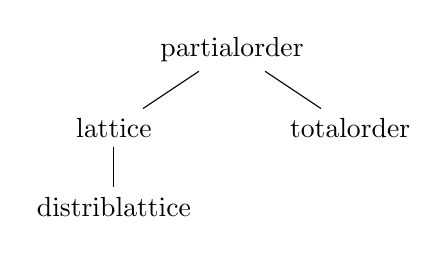
\begin{tikzpicture}
  \node (po) at (0,0) {\isa{partial{\isacharunderscore}order}};
  \node (lat) at (-1.5,-1) {\isa{lattice}};
  \node (dlat) at (-1.5,-2) {\isa{distrib{\isacharunderscore}lattice}};
  \node (to) at (1.5,-1) {\isa{total{\isacharunderscore}order}};
  \draw (po) -- (lat);
  \draw (lat) -- (dlat);
  \draw (po) -- (to);
%  \draw[->, dashed] (lat) -- (to);
\end{tikzpicture}
} \\
\subfigure[Total orders are lattices]{
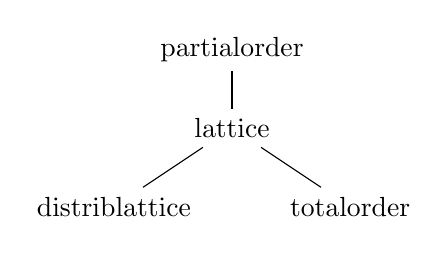
\begin{tikzpicture}
  \node (po) at (0,0) {\isa{partial{\isacharunderscore}order}};
  \node (lat) at (0,-1) {\isa{lattice}};
  \node (dlat) at (-1.5,-2) {\isa{distrib{\isacharunderscore}lattice}};
  \node (to) at (1.5,-2) {\isa{total{\isacharunderscore}order}};
  \draw (po) -- (lat);
  \draw (lat) -- (dlat);
  \draw (lat) -- (to);
%  \draw[->, dashed] (dlat) -- (to);
\end{tikzpicture}
} \quad
\subfigure[Total orders are distributive lattices]{
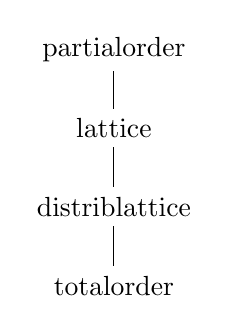
\begin{tikzpicture}
  \node (po) at (0,0) {\isa{partial{\isacharunderscore}order}};
  \node (lat) at (0,-1) {\isa{lattice}};
  \node (dlat) at (0,-2) {\isa{distrib{\isacharunderscore}lattice}};
  \node (to) at (0,-3) {\isa{total{\isacharunderscore}order}};
  \draw (po) -- (lat);
  \draw (lat) -- (dlat);
  \draw (dlat) -- (to);
\end{tikzpicture}
}
\end{center}
\hrule
\caption{Hierarchy of Lattice Locales.}
\label{fig:lattices}
\end{figure}%
\end{isamarkuptext}%
\isamarkuptrue%
%
\isamarkupsection{Changing the Locale Hierarchy%
}
\isamarkuptrue%
%
\begin{isamarkuptext}%
\label{sec:changing-the-hierarchy}

  Total orders are lattices.  Hence, by deriving the lattice
  axioms for total orders, the hierarchy may be changed
  and \isa{lattice} be placed between \isa{partial{\isacharunderscore}order}
  and \isa{total{\isacharunderscore}order}, as shown in Figure~\ref{fig:lattices}(b).
  Changes to the locale hierarchy may be declared
  with the \isakeyword{interpretation} command.%
\end{isamarkuptext}%
\isamarkuptrue%
%
\isadelimvisible
\ \ %
\endisadelimvisible
%
\isatagvisible
\isacommand{sublocale}\isamarkupfalse%
\ total{\isacharunderscore}order\ {\isasymsubseteq}\ lattice%
\begin{isamarkuptxt}%
This enters the context of locale \isa{total{\isacharunderscore}order}, in
  which the goal \begin{isabelle}%
\ {\isadigit{1}}{\isachardot}\ lattice\ op\ {\isasymsqsubseteq}%
\end{isabelle} must be shown.  First, the
  locale predicate needs to be unfolded --- for example using its
  definition or by introduction rules
  provided by the locale package.  The methods \isa{intro{\isacharunderscore}locales}
  and \isa{unfold{\isacharunderscore}locales} automate this.  They are aware of the
  current context and dependencies between locales and automatically
  discharge goals implied by these.  While \isa{unfold{\isacharunderscore}locales}
  always unfolds locale predicates to assumptions, \isa{intro{\isacharunderscore}locales} only unfolds definitions along the locale
  hierarchy, leaving a goal consisting of predicates defined by the
  locale package.  Occasionally the latter is of advantage since the goal
  is smaller.

  For the current goal, we would like to get hold of
  the assumptions of \isa{lattice}, hence \isa{unfold{\isacharunderscore}locales}
  is appropriate.%
\end{isamarkuptxt}%
\isamarkuptrue%
\ \ \isacommand{proof}\isamarkupfalse%
\ unfold{\isacharunderscore}locales%
\begin{isamarkuptxt}%
Since both \isa{lattice} and \isa{total{\isacharunderscore}order}
  inherit \isa{partial{\isacharunderscore}order}, the assumptions of the latter are
  discharged, and the only subgoals that remain are the assumptions
  introduced in \isa{lattice} \begin{isabelle}%
\ {\isadigit{1}}{\isachardot}\ {\isasymAnd}x\ y{\isachardot}\ {\isasymexists}inf{\isachardot}\ is{\isacharunderscore}inf\ x\ y\ inf\isanewline
\ {\isadigit{2}}{\isachardot}\ {\isasymAnd}x\ y{\isachardot}\ {\isasymexists}sup{\isachardot}\ is{\isacharunderscore}sup\ x\ y\ sup%
\end{isabelle}
  The proof for the first subgoal is%
\end{isamarkuptxt}%
\isamarkuptrue%
\ \ \ \ \isacommand{fix}\isamarkupfalse%
\ x\ y\isanewline
\ \ \ \ \isacommand{from}\isamarkupfalse%
\ total\ \isacommand{have}\isamarkupfalse%
\ {\isachardoublequoteopen}is{\isacharunderscore}inf\ x\ y\ {\isacharparenleft}if\ x\ {\isasymsqsubseteq}\ y\ then\ x\ else\ y{\isacharparenright}{\isachardoublequoteclose}\isanewline
\ \ \ \ \ \ \isacommand{by}\isamarkupfalse%
\ {\isacharparenleft}auto\ simp{\isacharcolon}\ is{\isacharunderscore}inf{\isacharunderscore}def{\isacharparenright}\isanewline
\ \ \ \ \isacommand{then}\isamarkupfalse%
\ \isacommand{show}\isamarkupfalse%
\ {\isachardoublequoteopen}{\isasymexists}inf{\isachardot}\ is{\isacharunderscore}inf\ x\ y\ inf{\isachardoublequoteclose}\ \isacommand{{\isachardot}{\isachardot}}\isamarkupfalse%
%
\begin{isamarkuptxt}%
The proof for the second subgoal is analogous and not
  reproduced here.%
\end{isamarkuptxt}%
\isamarkuptrue%
%
\endisatagvisible
{\isafoldvisible}%
%
\isadelimvisible
%
\endisadelimvisible
%
\isadeliminvisible
\ \ %
\endisadeliminvisible
%
\isataginvisible
\isacommand{next}\isamarkupfalse%
\isanewline
\ \ \ \ \isacommand{fix}\isamarkupfalse%
\ x\ y\isanewline
\ \ \ \ \isacommand{from}\isamarkupfalse%
\ total\ \isacommand{have}\isamarkupfalse%
\ {\isachardoublequoteopen}is{\isacharunderscore}sup\ x\ y\ {\isacharparenleft}if\ x\ {\isasymsqsubseteq}\ y\ then\ y\ else\ x{\isacharparenright}{\isachardoublequoteclose}\isanewline
\ \ \ \ \ \ \isacommand{by}\isamarkupfalse%
\ {\isacharparenleft}auto\ simp{\isacharcolon}\ is{\isacharunderscore}sup{\isacharunderscore}def{\isacharparenright}\isanewline
\ \ \ \ \isacommand{then}\isamarkupfalse%
\ \isacommand{show}\isamarkupfalse%
\ {\isachardoublequoteopen}{\isasymexists}sup{\isachardot}\ is{\isacharunderscore}sup\ x\ y\ sup{\isachardoublequoteclose}\ \isacommand{{\isachardot}{\isachardot}}\isamarkupfalse%
%
\endisataginvisible
{\isafoldinvisible}%
%
\isadeliminvisible
%
\endisadeliminvisible
%
\isadelimvisible
\ %
\endisadelimvisible
%
\isatagvisible
\isacommand{qed}\isamarkupfalse%
%
\endisatagvisible
{\isafoldvisible}%
%
\isadelimvisible
%
\endisadelimvisible
%
\begin{isamarkuptext}%
Similarly, total orders are distributive lattices.%
\end{isamarkuptext}%
\isamarkuptrue%
\ \ \isacommand{sublocale}\isamarkupfalse%
\ total{\isacharunderscore}order\ {\isasymsubseteq}\ distrib{\isacharunderscore}lattice\isanewline
%
\isadelimproof
\ \ %
\endisadelimproof
%
\isatagproof
\isacommand{proof}\isamarkupfalse%
\ unfold{\isacharunderscore}locales\isanewline
\ \ \ \ \isacommand{fix}\isamarkupfalse%
\ x\ y\ z\isanewline
\ \ \ \ \isacommand{show}\isamarkupfalse%
\ {\isachardoublequoteopen}x\ {\isasymsqinter}\ {\isacharparenleft}y\ {\isasymsqunion}\ z{\isacharparenright}\ {\isacharequal}\ x\ {\isasymsqinter}\ y\ {\isasymsqunion}\ x\ {\isasymsqinter}\ z{\isachardoublequoteclose}\ {\isacharparenleft}\isakeyword{is}\ {\isachardoublequoteopen}{\isacharquery}l\ {\isacharequal}\ {\isacharquery}r{\isachardoublequoteclose}{\isacharparenright}%
\begin{isamarkuptxt}%
Jacobson I, p.\ 462%
\end{isamarkuptxt}%
\isamarkuptrue%
\ \ \ \ \isacommand{proof}\isamarkupfalse%
\ {\isacharminus}\isanewline
\ \ \ \ \ \ \isacommand{{\isacharbraceleft}}\isamarkupfalse%
\ \isacommand{assume}\isamarkupfalse%
\ c{\isacharcolon}\ {\isachardoublequoteopen}y\ {\isasymsqsubseteq}\ x{\isachardoublequoteclose}\ {\isachardoublequoteopen}z\ {\isasymsqsubseteq}\ x{\isachardoublequoteclose}\isanewline
\ \ \ \ \ \ \ \ \isacommand{from}\isamarkupfalse%
\ c\ \isacommand{have}\isamarkupfalse%
\ {\isachardoublequoteopen}{\isacharquery}l\ {\isacharequal}\ y\ {\isasymsqunion}\ z{\isachardoublequoteclose}\isanewline
\ \ \ \ \ \ \ \ \ \ \isacommand{by}\isamarkupfalse%
\ {\isacharparenleft}metis\ c\ join{\isacharunderscore}connection{\isadigit{2}}\ join{\isacharunderscore}related{\isadigit{2}}\ meet{\isacharunderscore}related{\isadigit{2}}\ total{\isacharparenright}\isanewline
\ \ \ \ \ \ \ \ \isacommand{also}\isamarkupfalse%
\ \isacommand{from}\isamarkupfalse%
\ c\ \isacommand{have}\isamarkupfalse%
\ {\isachardoublequoteopen}{\isachardot}{\isachardot}{\isachardot}\ {\isacharequal}\ {\isacharquery}r{\isachardoublequoteclose}\ \isacommand{by}\isamarkupfalse%
\ {\isacharparenleft}metis\ meet{\isacharunderscore}related{\isadigit{2}}{\isacharparenright}\isanewline
\ \ \ \ \ \ \ \ \isacommand{finally}\isamarkupfalse%
\ \isacommand{have}\isamarkupfalse%
\ {\isachardoublequoteopen}{\isacharquery}l\ {\isacharequal}\ {\isacharquery}r{\isachardoublequoteclose}\ \isacommand{{\isachardot}}\isamarkupfalse%
\ \isacommand{{\isacharbraceright}}\isamarkupfalse%
\isanewline
\ \ \ \ \ \ \isacommand{moreover}\isamarkupfalse%
\isanewline
\ \ \ \ \ \ \isacommand{{\isacharbraceleft}}\isamarkupfalse%
\ \isacommand{assume}\isamarkupfalse%
\ c{\isacharcolon}\ {\isachardoublequoteopen}x\ {\isasymsqsubseteq}\ y\ {\isasymor}\ x\ {\isasymsqsubseteq}\ z{\isachardoublequoteclose}\isanewline
\ \ \ \ \ \ \ \ \isacommand{from}\isamarkupfalse%
\ c\ \isacommand{have}\isamarkupfalse%
\ {\isachardoublequoteopen}{\isacharquery}l\ {\isacharequal}\ x{\isachardoublequoteclose}\isanewline
\ \ \ \ \ \ \ \ \ \ \isacommand{by}\isamarkupfalse%
\ {\isacharparenleft}metis\ join{\isacharunderscore}connection{\isadigit{2}}\ join{\isacharunderscore}related{\isadigit{2}}\ meet{\isacharunderscore}connection\ total\ trans{\isacharparenright}\isanewline
\ \ \ \ \ \ \ \ \isacommand{also}\isamarkupfalse%
\ \isacommand{from}\isamarkupfalse%
\ c\ \isacommand{have}\isamarkupfalse%
\ {\isachardoublequoteopen}{\isachardot}{\isachardot}{\isachardot}\ {\isacharequal}\ {\isacharquery}r{\isachardoublequoteclose}\isanewline
\ \ \ \ \ \ \ \ \ \ \isacommand{by}\isamarkupfalse%
\ {\isacharparenleft}metis\ join{\isacharunderscore}commute\ join{\isacharunderscore}related{\isadigit{2}}\ meet{\isacharunderscore}connection\ meet{\isacharunderscore}related{\isadigit{2}}\ total{\isacharparenright}\isanewline
\ \ \ \ \ \ \ \ \isacommand{finally}\isamarkupfalse%
\ \isacommand{have}\isamarkupfalse%
\ {\isachardoublequoteopen}{\isacharquery}l\ {\isacharequal}\ {\isacharquery}r{\isachardoublequoteclose}\ \isacommand{{\isachardot}}\isamarkupfalse%
\ \isacommand{{\isacharbraceright}}\isamarkupfalse%
\isanewline
\ \ \ \ \ \ \isacommand{moreover}\isamarkupfalse%
\ \isacommand{note}\isamarkupfalse%
\ total\isanewline
\ \ \ \ \ \ \isacommand{ultimately}\isamarkupfalse%
\ \isacommand{show}\isamarkupfalse%
\ {\isacharquery}thesis\ \isacommand{by}\isamarkupfalse%
\ blast\isanewline
\ \ \ \ \isacommand{qed}\isamarkupfalse%
\isanewline
\ \ \isacommand{qed}\isamarkupfalse%
%
\endisatagproof
{\isafoldproof}%
%
\isadelimproof
%
\endisadelimproof
%
\begin{isamarkuptext}%
The locale hierarchy is now as shown in Figure~\ref{fig:lattices}(c).%
\end{isamarkuptext}%
\isamarkuptrue%
%
\isadelimtheory
%
\endisadelimtheory
%
\isatagtheory
\isacommand{end}\isamarkupfalse%
%
\endisatagtheory
{\isafoldtheory}%
%
\isadelimtheory
%
\endisadelimtheory
\isanewline
\end{isabellebody}%
%%% Local Variables:
%%% mode: latex
%%% TeX-master: "root"
%%% End:
